
% ============================================================
% CHAPTER 03
% UNITY AND PLURALITY
% Book I: Ontology of Viability
% ============================================================

\chapter{Unity and Plurality}
\label{ch:unity-and-plurality}

% ------------------------------------------------------------
% CHAPTER METADATA
% ------------------------------------------------------------

\newcommand{\ChapterThreeTitle}{Unity and Plurality}
\newcommand{\ChapterThreeID}{VS.B01.P01.C03}

% ------------------------------------------------------------
% OPENING QUOTATION
% ------------------------------------------------------------

\begin{quote}
Unity and plurality are not conclusions that may be
established merely by counting components, manifestations,
or relations. Their ontological significance depends on
what is said to be one or many, and in what respect.
\end{quote}

% ------------------------------------------------------------
% CHAPTER INTRODUCTION
% ------------------------------------------------------------

\section*{Introduction}
\addcontentsline{toc}{section}{Introduction}

The preceding chapters established two foundational
dimensions of the ontology of identity. The first examined
the ontological relation between being and identity,
while the second investigated invariance as a distinct
problem concerning the persistence of determinate aspects
in relation to specified domains of change.

The present chapter addresses another fundamental
ontological problem: the relation between unity and
plurality.

The question of unity and plurality arises whenever an
existent, or a domain of existence, is considered in
terms of its possible oneness, multiplicity, or internal
differentiation. An existent may exhibit multiple
determinations, components, relations, or manifestations.
However, the presence of such multiplicity does not
immediately establish that the existent possesses multiple
identities.

Conversely, the apparent unity of an existent does not,
by itself, establish that its identity is numerically
singular. The unity of an aggregate, the unity of a source,
the unity of an organized composition, and the unity
of identity constitute distinguishable problems whose
relations require examination.

Accordingly, this chapter does not begin by assuming
that every existent necessarily possesses exactly one
identity. Nor does it assume that plurality within an
existent necessarily entails a plurality of identities.
Both possibilities remain subject to ontological analysis.

For the purposes of this inquiry, several distinctions
must be maintained.

First, unity must be distinguished from singularity.
The fact that something is considered as one does not
necessarily establish that it is numerically singular
in every relevant ontological respect.

Second, unity of identity must be distinguished from
unity of source and unity of aggregate. These expressions
refer to different possible grounds or subjects of unity
and cannot be treated as interchangeable.

Third, plurality of components, determinations, relations,
or manifestations must be distinguished from plurality
of identities. Multiplicity at one ontological level
does not automatically establish multiplicity at another.

Fourth, identity must be distinguished from composition.
An existent may possess a complex composition without
its identity being reducible to that composition. Likewise,
the existence of multiple components does not, by itself,
settle whether the relevant existent is one or many in
the respect under consideration.

These distinctions are not introduced to impose a
predetermined solution. Their purpose is to prevent
different ontological questions from being collapsed
into a single and insufficiently specified claim.

The analysis also requires attention to the subject
of every assertion of unity or plurality. Whenever
something is described as one or many, it is necessary
to determine what the assertion concerns: an identity,
a source, an aggregate, a composition, a relation,
a manifestation, or another ontological determination.

Without identifying the relevant subject and respect,
the assertion of unity or plurality remains ambiguous.

The preceding chapter's analysis of invariance is relevant
to this inquiry, but invariance cannot serve as a substitute
for the analysis of unity and plurality. The persistence
of an invariant aspect does not establish numerical
unity of identity. Similarly, the absence of an identified
invariant does not establish ontological plurality.

The present chapter therefore approaches unity and
plurality as an independent ontological problem. It
examines their possible relations to identity, source,
aggregate, composition, and multiplicity without reducing
one concept to another.

The chapter proceeds from the formulation of the
ontological problem to the examination of unity of
identity, unity of source and aggregate, plurality of
identities, and plurality in relation to composition.
It subsequently considers multiplicity, the distinction
between unity and singularity, and the limits of what
can be established through these concepts.

The purpose is not to produce a premature universal
definition of unity or plurality. Rather, it is to clarify
the conditions under which claims concerning oneness
and multiplicity may be ontologically meaningful,
and to identify the distinctions necessary for their
further development within the ontology of viability.

% ------------------------------------------------------------
% SECTION 01
% ------------------------------------------------------------


% =============================================================================
% Section 01 — The Ontological Problem of Unity and Plurality
% Book I — Ontology of Viability
% Chapter 03 — Unity and Plurality
%
% Purpose:
%   To formulate the ontological problem of unity and plurality,
%   identify its principal conceptual dimensions, and establish
%   the distinctions required for its subsequent examination.
%
% Conceptual Policy:
%   1. Unity and plurality are treated as ontological problems,
%      not merely logical, linguistic, or epistemic problems.
%   2. Unity is not initially reduced to numerical singularity,
%      aggregation, structural coherence, or invariance.
%   3. Plurality is not initially reduced to plurality of parts,
%      manifestations, relations, or identities.
%   4. The relation between identity and unity remains open
%      for explicit examination in the following sections.
%   5. No assumption is made that every existent has exactly
%      one identity or that plurality necessarily entails
%      multiple identities.
% =============================================================================

\section{The Ontological Problem of Unity and Plurality}
\label{sec:ontological-problem-of-unity-and-plurality}

\subsection{The Question of Unity and Plurality}

The relation between unity and plurality constitutes a fundamental
problem in ontology. Every account of existence that encounters
determinate existents must also confront the question of how
something is one, how multiplicity is possible, and how unity
and plurality can belong to the same ontological field without
being confused or prematurely reduced to one another.

The problem is not exhausted by the observation that reality
contains many things. Nor is it resolved by asserting that each
thing is, in some respect, one. Such statements identify the
presence of unity and plurality but do not explain their
ontological status or their relation.

The central question is therefore not simply whether unity and
plurality exist, but what it means for an existent to possess
unity, what it means for multiplicity to obtain, and under what
conditions these determinations can belong to the same existent
or to related existents.

An existent may be considered one while also exhibiting internal
differentiation, multiple determinations, distinct components,
various relations, or several modes of manifestation. Conversely,
a plurality of existents may be considered together as a group,
collection, or organized whole. These situations are not
ontologically identical. They involve different senses of unity
and plurality, and their differences require explicit analysis.

The first task of this chapter is consequently to prevent the
problem from being reduced to a single relation between one
and many. Unity and plurality are not sufficiently understood
through a numerical opposition alone. Their ontological
significance depends on what is unified, what is multiple,
and the respect in which either determination is asserted.

\subsection{Unity as an Ontological Determination}

Unity cannot be treated merely as a numerical description
superimposed upon an existent from an external standpoint.
The question of unity concerns the ontological determination
of an existent as one, rather than only the manner in which
it is counted, named, classified, or considered.

To call something one may indicate different claims:

\begin{itemize}
    \item that an existent possesses a unified identity;
    \item that several components belong to one organized whole;
    \item that multiple determinations belong to one existent;
    \item that a plurality is collected under a common designation;
    \item that an existent is numerically distinct from another;
    \item that a configuration exhibits a certain degree of
    structural coherence.
\end{itemize}

These claims must not be assumed to express one and the same
ontological condition.

A collection can be one collection without necessarily
constituting one identity. An organized whole can possess
structural unity without that unity being identical to the
identity of its components or to the identity of the whole.
Likewise, the numerical distinction of an existent from another
does not, by itself, explain the ontological constitution of
its unity.

Unity must therefore be investigated according to the
ontological determination to which it refers. Its meaning
cannot be established solely by the grammatical or numerical
form of a statement.

The present section does not yet provide a complete definition
of unity. It establishes that unity is a problem requiring
differentiation among several possible ontological senses.

\subsection{Plurality as an Ontological Determination}

Plurality is equally resistant to a single undifferentiated
interpretation.

The presence of more than one component does not necessarily
establish the presence of more than one identity. The presence
of several relations does not necessarily establish several
existents. The multiplicity of manifestations does not,
without further argument, establish a multiplicity of the
identities manifested.

Plurality may concern different ontological determinations,
including:

\begin{itemize}
    \item plurality of existents;
    \item plurality of identities;
    \item plurality of components;
    \item plurality of determinations;
    \item plurality of relations;
    \item plurality of manifestations;
    \item plurality of configurations or compositions.
\end{itemize}

These forms of plurality cannot be treated as interchangeable.
Each concerns a different possible object of multiplicity
and requires its own ontological examination.

In particular, plurality of components and plurality of
identities must remain distinct questions. A composed existent
may contain multiple components without the number of its
components determining the number of identities involved.
Similarly, the multiplicity of manifestations associated with
an identity cannot be converted into a plurality of identities
without establishing an additional ontological criterion.

Plurality must therefore be specified according to what is
multiple. An assertion that something is multiple remains
ontologically incomplete until the relevant multiplicity
and its domain have been identified.

\subsection{The Apparent Opposition Between the One and the Many}

Unity and plurality are frequently presented as opposing
determinations. If something is one, it may appear that it
cannot also be many; if something is many, it may appear
that it cannot possess unity.

This opposition, however, is not yet an established ontological
contradiction. It may result from treating distinct senses
of unity and plurality as if they referred to the same
determination in the same respect.

For example, the unity of an existent and the plurality
of its components are not necessarily contradictory claims.
The first concerns the existent as a unified ontological
referent; the second concerns the multiplicity of elements
associated with its composition.

Likewise, the unity of an identity and the plurality of its
manifestations cannot be declared contradictory merely
because the terms one and many are applied within the same
ontological situation. The relevant question is whether
they refer to the same ontological subject and the same
determination, or to distinct but related determinations.

This distinction does not automatically resolve every
problem concerning unity and plurality. It only establishes
that an apparent opposition cannot be treated as a genuine
contradiction without first specifying the terms of the
opposition.

A valid ontological analysis must therefore distinguish
between:

\begin{enumerate}
    \item a genuine incompatibility between two determinations;
    \item the coexistence of distinct determinations within
    one existent;
    \item the relation between a unified existent and a plurality
    associated with it;
    \item the unity attributed to a plurality considered as
    a collection or organized whole.
\end{enumerate}

The distinction between these situations is a condition
of the inquiry, not its final conclusion.

\subsection{The Problem of the Subject of Unity}

Any claim concerning unity requires clarification of its
subject. The expression ``one'' does not identify, by itself,
what possesses unity or what kind of unity is being asserted.

The subject of unity may be an existent, an identity, a
composition, a structure, a relation, or an aggregate.
These subjects are not interchangeable.

The unity of an existent must not be assumed to be identical
to the unity of its composition. Nor can the unity of a
structure automatically be identified with the unity of
the existent whose determinations it organizes.

The same difficulty arises when plurality is considered.
A plurality may belong to an existent as its components,
to an identity through its manifestations, or to a domain
through the presence of several distinct existents.

Consequently, the ontological analysis of unity and plurality
requires two questions to be kept separate:

\begin{enumerate}
    \item What is the subject to which unity or plurality
    is attributed?
    \item What ontological determination is being described
    as unified or multiple?
\end{enumerate}

Failure to distinguish these questions leads to the
unwarranted transfer of properties from one ontological
subject to another.

The unity of an aggregate, for example, cannot establish
the unity of an identity merely because the aggregate
is considered one object. Likewise, the plurality of
components cannot establish the plurality of identities
merely because several components are present.

\subsection{Unity, Identity, and Numerical Distinction}

The problem of unity is closely related to identity,
but the two concepts must not be identified without
argument.

The preceding chapter established that invariance does
not constitute identity and that the preservation of
invariant determinations cannot independently establish
numerical identity. The present inquiry must preserve
the same conceptual discipline: unity cannot be assumed
to provide a complete definition or criterion of identity.

The unity of identity concerns the identity as one.
The numerical distinction between identities concerns
whether two identity-referents are numerically distinct.
The unity of a composition concerns the organization
or belonging together of its constituents.

These questions are related, but they are not equivalent.

In particular, the statement that an identity is one
does not yet explain whether an existent can possess
multiple identities, whether distinct identities can
belong to one composed existent, or whether one identity
can be associated with multiple manifestations.

Those questions require separate examination.

The present section therefore adopts no unrestricted
principle according to which every existent must possess
exactly one identity. It also does not assume that
multiple identities can be attributed to one existent
without qualification. Both positions require further
ontological argument.

\subsection{Unity and Singularity}

Unity must also be distinguished from singularity.

Singularity may refer to numerical uniqueness, the
non-duplication of an existent, or its distinction from
other existents. Unity, by contrast, concerns the
ontological condition under which something is one.

Although these concepts may coincide in particular
cases, their meanings are not identical.

An existent may be considered one without the concept
of unity thereby explaining its numerical uniqueness.
Conversely, a plurality may possess some form of unity
without becoming numerically singular in every relevant
respect.

The fact that a collection is treated as one collection,
for example, does not make its components numerically
singular. Similarly, the numerical distinctness of an
existent does not by itself explain the unity of its
identity or composition.

The distinction is essential because an account that
reduces unity to singularity risks treating every question
of unity as a question of counting. Such a reduction
would leave unexplained the ontological relations among
identity, composition, multiplicity, and the unity of
organized wholes.

The non-equivalence of unity and singularity will be
examined directly in Section~\ref{sec:non-equivalence-of-unity-and-singularity}.

\subsection{Unity and Composition}

Composition introduces a further dimension of the problem.

An existent may possess components, and those components
may stand in determinate relations to one another.
Their organization may constitute a composition or
an organized whole.

However, the unity of a composition cannot be assumed
to be identical to the unity of an identity.

The fact that several components belong to one composition
does not establish that they constitute one identity in
every ontological respect. Equally, the fact that a
composition undergoes changes in its components does
not, without further argument, determine whether its
identity remains, changes, or ceases.

The relation between unity and composition must therefore
be investigated without presupposing that the whole is
merely the sum of its parts or that the unity of the
whole is reducible to the relations among those parts.

This inquiry also requires distinguishing the unity
of an aggregate from the unity of an existent whose
composition is ontologically constitutive of it.

The distinction between these possibilities will be
developed in Sections~\ref{sec:unity-of-source-and-aggregate}
and~\ref{sec:plurality-and-composition}.

\subsection{The Problem of Plurality Within and Beyond an Existent}

Plurality can be considered internally or externally,
but this distinction must not be mistaken for a complete
classification of multiplicity.

Internal plurality concerns multiplicity attributed
to or present within an existent. It may involve
components, determinations, relations, or other
ontological differentiations.

External plurality concerns the presence of several
distinct existents within a wider domain or relation.

Neither category, by itself, determines the number
of identities involved.

Internal plurality does not necessarily entail
multiple identities, while external plurality
cannot be adequately described merely by counting
components or manifestations.

Moreover, the distinction between internal and external
plurality depends on the ontological boundaries and
determinations under examination. These boundaries
must not be assumed to be self-evident in every case.

The analysis must therefore remain attentive to the
difference between:

\begin{itemize}
    \item multiplicity within one existent;
    \item multiplicity among distinct existents;
    \item multiplicity among identities;
    \item multiplicity among manifestations;
    \item multiplicity generated or constituted through
    composition and relation.
\end{itemize}

The following sections will examine these distinctions
without assuming that one category can be reduced
to another.

\subsection{The Ontological Stakes of the Problem}

The problem of unity and plurality affects several
fundamental questions of ontology.

First, it concerns the status of identity. If unity
is reduced to aggregation, the identity of an existent
risks being treated as nothing more than the collection
of its constituents. If unity is reduced to structure,
identity risks being identified with a particular
organization of determinations. Neither reduction
can be accepted without an independent argument.

Second, the problem concerns the status of composition.
If plurality is treated as incompatible with unity,
the ontological possibility of composed existents
becomes difficult to explain. If unity is attributed
to every collection without qualification, however,
the distinction between an aggregate and an ontologically
unified existent disappears.

Third, the problem concerns the distinction among
different identities. If plurality of components,
relations, or manifestations is automatically interpreted
as plurality of identities, the number of identities
will be determined by categories that do not necessarily
correspond to identity itself.

Fourth, the problem concerns the limits of ontological
claims. Neither unity nor plurality should be extended
beyond the conditions under which it has been established.
A claim concerning one domain or determination cannot
automatically be generalized to every domain or
determination.

The chapter must therefore establish not merely that
unity and plurality coexist, but the conditions under
which particular forms of unity and plurality can
be attributed to particular ontological subjects.

\subsection{Methodological Requirements for the Inquiry}

The subsequent examination of unity and plurality
will proceed according to several methodological
requirements.

\begin{enumerate}
    \item \textbf{Specification of the subject:}
    Every claim of unity or plurality must identify
    the existent, identity, composition, aggregate,
    or other ontological subject under consideration.

    \item \textbf{Specification of the determination:}
    The analysis must identify whether unity or plurality
    concerns identity, composition, structure, relation,
    manifestation, or another determination.

    \item \textbf{Non-reduction:}
    Unity must not be reduced in advance to singularity,
    aggregation, structural coherence, or invariance.
    Plurality must not be reduced in advance to the
    plurality of components or identities.

    \item \textbf{Respect for ontological distinctions:}
    Distinctions established in the preceding chapters,
    especially those concerning identity, determination,
    composition, and invariance, must remain operative.

    \item \textbf{Separation of established claims and open questions:}
    A conceptual distinction does not automatically
    establish a complete ontological theory. Where
    the conditions of a claim remain unresolved, the
    question must remain open.

    \item \textbf{No premature universalization:}
    The analysis must not assume that every existent,
    every composition, or every domain exhibits one
    and the same form of unity or plurality.
\end{enumerate}

These requirements establish the conditions under
which the chapter can proceed without confusing
different ontological levels or treating a limited
claim as a universal principle.

\subsection{Scope of the Present Section}

The present section has formulated the ontological
problem of unity and plurality and identified the
principal distinctions required for its examination.

It has not yet established a complete definition
of unity, a universal account of plurality, or a
final criterion for determining the number of
identities associated with an existent.

Nor has it established that unity is always prior
to plurality, that plurality is always derived
from unity, or that one can be reduced to the other.

The following sections will examine these questions
in a determinate order.

Section~\ref{sec:unity-of-identity} investigates
the unity of identity.

Section~\ref{sec:unity-of-source-and-aggregate}
examines the distinction between unity of source
and unity of aggregate.

Section~\ref{sec:plurality-of-identities} addresses
the possibility and ontological status of plurality
of identities.

Section~\ref{sec:plurality-and-composition} examines
the relation between plurality and composition,
while Section~\ref{sec:identity-and-multiplicity}
investigates the broader relation between identity
and multiplicity.

Finally, the chapter distinguishes unity from
singularity, establishes the limits of claims
concerning unity and plurality, and synthesizes
the results of the inquiry.

The governing methodological commitment is that
unity and plurality must be understood through
their respective ontological subjects and
determinations. Neither can be defined adequately
by reducing it to the other, and neither can be
treated as a universal explanation of the
ontological constitution of existents.


% ------------------------------------------------------------
% SECTION 02
% ------------------------------------------------------------

% =============================================================================
% Section 02 — Unity of Identity
% Book I — Ontology of Viability
% Chapter 03 — Unity and Plurality
%
% Purpose:
%   To examine the ontological meaning and scope of the unity
%   of identity without reducing identity to singularity,
%   numerical indivisibility, unity of source, composition,
%   or invariance.
%
% Conceptual Policy:
%   1. Unity of identity must be distinguished from the unity
%      of an aggregate and from the unity of a source.
%   2. Unity must not be equated with singularity.
%   3. The unity of identity must not be derived from the
%      invariance of a configuration or set of determinations.
%   4. The possibility of plurality of identities must remain
%      open and must not be excluded by definition.
%   5. No universal assumption that every existent possesses
%      exactly one identity is adopted.
%
% =============================================================================

\section{Unity of Identity}
\label{sec:unity-of-identity}

% -----------------------------------------------------------------------------
\subsection{The Meaning of Unity in the Context of Identity}

The question of unity acquires a distinct ontological significance
when it is considered in relation to identity.

An existent may be described as unified in different respects.
Its determinations may form an organized configuration;
its components may constitute an aggregate;
its manifestations may be related to a common source;
or its existence may be considered under a single identity.
These descriptions concern different possible forms of unity
and cannot be treated as interchangeable.

The present section is concerned specifically with the
\emph{unity of identity}.
It therefore asks whether, and in what sense, identity may
constitute a unity, rather than merely whether an existent
possesses an organized structure or an identifiable source.

Unity of identity is not simply the observation that several
determinations belong to one existent.
Nor is it equivalent to the fact that several components
participate in one composition.
The ontological question concerns the unity attributable
to identity itself.

This distinction is necessary because the unity of an existent
in one respect does not automatically establish its unity
in every other respect.

A composition may be unified while the question of its
identity remains unresolved.
A plurality of manifestations may be related without
thereby determining whether they belong to one identity
or to several.
Likewise, a common source may provide a basis for examining
unity without proving that every manifestation associated
with that source possesses the same identity.

Unity of identity must therefore be examined as a distinct
ontological determination.

% -----------------------------------------------------------------------------
\subsection{Unity Is Not an Additional Property of Identity}

Unity should not be understood as an independent property
that is externally attached to an already constituted identity.

If identity is ontologically inseparable from being,
then unity cannot be treated as a merely supplementary
attribute that is added to identity after its constitution.

Such an interpretation would presuppose that identity
is first constituted independently and subsequently
receives unity as an additional determination.
This would introduce an artificial separation between
identity and a possible mode of its ontological unity.

However, recognizing this inseparability does not establish
that every identity must be singular in every possible respect.
Nor does it demonstrate that the unity of identity can be
adequately described through a single universal formula.

The claim that unity is not externally added to identity
must be distinguished from the stronger claim that every
existent necessarily possesses exactly one identity.

The former concerns the ontological relation between
identity and unity.
The latter concerns the number of identities that may
belong to an existent.

These are different questions and require different arguments.

Accordingly, unity of identity is considered here as an
ontological problem concerning the mode in which identity
is unified, rather than as a supplementary attribute
or a predetermined numerical condition.

% -----------------------------------------------------------------------------
\subsection{Unity of Identity and Numerical Singularity}

Unity of identity must be distinguished from numerical
singularity.

Numerical singularity concerns whether something is one
in number rather than more than one.
Unity, however, may concern the ontological coherence
or unity of identity without necessarily settling
the numerical question.

An existent may be numerically one under a particular
description while the ontological status of its identity
remains open.

Conversely, the possibility that an existent involves
more than one identity cannot be excluded merely because
it is treated as one object, one organism, one system,
or one material aggregate in a particular domain.

The numerical designation of an existent does not,
by itself, determine the number or mode of its identities.

This distinction prevents a transition from numerical
description to ontological conclusion without sufficient
argument.

To call something one does not automatically establish
that its identity is singular.
Likewise, to identify several components or manifestations
does not automatically establish that several identities
are present.

The relation between unity and singularity is examined
more directly in Section~\ref{sec:non-equivalence-of-unity-and-singularity}.
For the present inquiry, it is sufficient to establish
that numerical singularity cannot serve as an unquestioned
definition or proof of unity of identity.

% -----------------------------------------------------------------------------
\subsection{Unity of Identity and Unity of Source}

The unity of identity must also be distinguished from
the unity of source.

Several manifestations may be associated with one source.
This relation may provide an important basis for examining
their ontological connection.
Nevertheless, the unity of their source does not
automatically determine the unity of their identities.

The inference from one source to one identity requires
additional ontological justification.

A common source may be relevant to the constitution,
generation, or manifestation of several entities.
Yet the relation between source and identity cannot
be settled merely by counting sources or manifestations.

It is therefore necessary to distinguish at least
two questions:

\begin{enumerate}
    \item Whether several manifestations are related
    to one source.

    \item Whether those manifestations belong to one
    identity or involve a plurality of identities.
\end{enumerate}

The first question concerns the ontological relation
of manifestations to their source.
The second concerns the unity or plurality of identity.

Neither question can be substituted for the other.

This distinction also prevents the reduction of identity
to origin.
An existent cannot be assigned an identity solely by
establishing where it originates, unless the ontological
relevance of that origin to identity has independently
been demonstrated.

The distinction between unity of source and unity
of aggregate is developed in
Section~\ref{sec:unity-of-source-and-aggregate}.

% -----------------------------------------------------------------------------
\subsection{Unity of Identity and Composition}

The unity of identity must not be reduced to the unity
of composition.

Composition concerns the relation among components
that constitute an organized whole.
It may involve material, structural, functional,
or other forms of organization.

Identity, however, is not exhausted by the arrangement
or aggregation of components.

A composed existent may exhibit a high degree of
structural integration without this fact alone establishing
the ontological unity of its identity.

Likewise, changes in composition do not necessarily
establish the emergence of a new identity.
Nor does the preservation of a composition necessarily
prove the persistence of one identity.

The relation between identity and composition therefore
requires an analysis that does not assume either that
composition determines identity or that identity
is independent of every compositional condition.

The relevant question is not whether composition
is ontologically irrelevant.
Rather, it is whether and under what conditions
compositional relations contribute to the unity
of identity.

This question is treated separately in
Section~\ref{sec:plurality-and-composition}.

% -----------------------------------------------------------------------------
\subsection{Unity of Identity and Invariance}

Unity of identity must also be distinguished from
the preservation of invariant determinations.

An existent may preserve certain determinations
under transformation.
Such preservation may establish an invariant relation
within a specified domain and with respect to
a specified transformation.

However, the presence of invariants does not by itself
establish that the existent possesses one unified identity.

An invariant may be shared by distinct existents.
Different identities may preserve similar or identical
determinations.
Conversely, an existent may undergo transformations
in which previously identified invariants cease to hold
without this fact alone demonstrating the disappearance
of its identity.

The unity of identity therefore cannot be inferred
solely from the persistence of invariant features.

This does not mean that invariance is irrelevant
to the examination of identity.
It means that invariance and unity of identity
answer different ontological questions.

Invariance concerns what remains preserved under
a specified transformation.
Unity of identity concerns the ontological unity
attributable to identity.

Their possible relations must be established
without reducing one to the other.

The distinction developed in Chapter~\ref{ch:invariance}
is therefore presupposed here as a conceptual constraint,
not as a complete solution to the problem of unity.

% -----------------------------------------------------------------------------
\subsection{Unity and the Plurality of Determinations}

An existent may involve a plurality of determinations.
These determinations may differ in kind, mode,
relation, or ontological role.

The presence of such plurality does not automatically
negate the possibility of unity of identity.

A plurality of determinations may be compatible
with the unity of an identity.
However, this compatibility must not be interpreted
as proof that all plural determinations necessarily
belong to one identity.

The question concerns the ontological relation
between determinations and identity.

It is therefore necessary to avoid two opposite reductions.

The first reduction assumes that plurality of
determinations necessarily implies plurality
of identities.

The second assumes that the unity of an existent
necessarily absorbs every plurality of determinations
into one identity.

Neither inference is justified without further analysis.

The plurality of determinations may concern the
internal constitution, manifestation, or relations
of an existent.
Whether such plurality also involves a plurality
of identities is a separate question.

The distinction between unity and plurality must
therefore be maintained at the level of the subject
and the respect under consideration.

% -----------------------------------------------------------------------------
\subsection{Unity Without Reduction to Homogeneity}

Unity of identity must not be confused with homogeneity.

Homogeneity concerns similarity or sameness among
elements, determinations, or features in a specified
respect.

Unity, by contrast, cannot be defined merely as the
absence of difference.

An existent may involve differentiated determinations
without those differences necessarily destroying
the unity of its identity.

Likewise, the presence of similar or homogeneous
features does not establish that several entities
possess one identity.

Similarity is not identity, and difference is not
by itself proof of distinct identity.

This distinction is important because a theory that
defines unity through homogeneity risks treating
internal differentiation as a threat to identity.

Such a theory would make the possibility of unity
depend on the reduction or elimination of difference.

The present inquiry does not adopt this assumption.

Unity and difference must be examined in relation
to one another without presuming that one necessarily
abolishes the other.

The ontological status of difference in relation
to identity is considered further in the analysis
of unity and plurality.

% -----------------------------------------------------------------------------
\subsection{The Question of the Subject of Unity}

Every claim of unity requires clarification of
the subject to which unity is attributed.

An assertion that something is unified remains
incomplete unless it specifies what is being
considered as unified.

The subject may be an existent, an identity,
a source, an aggregate, a composition,
a configuration of determinations,
or a set of manifestations.

These subjects are not interchangeable.

For example, the unity of a material aggregate
does not automatically establish the unity
of the identity of that aggregate.
Similarly, the unity of a source does not
automatically establish the unity of the identities
associated with its manifestations.

The ontological subject of unity must therefore
be distinguished from the elements, relations,
or determinations through which unity is expressed.

This requirement also applies to claims of plurality.
A plurality of components, relations, or manifestations
cannot be transferred without argument into
a claim concerning a plurality of identities.

The examination of unity must consequently specify:

\begin{enumerate}
    \item The subject whose unity is being asserted.
    \item The ontological respect in which unity is asserted.
    \item The relations or determinations relevant
    to that unity.
    \item The limits beyond which the claim of unity
    cannot be extended.
\end{enumerate}

These requirements prevent the unrestricted use
of the term unity across different ontological levels.

% -----------------------------------------------------------------------------
\subsection{The Possibility of Plurality Within an Existent}

The examination of unity of identity must leave open
the possibility that an existent may involve a plurality
of identities.

This possibility cannot be rejected merely by assuming
that the unity of an existent entails the singularity
of its identity.

At the same time, the possibility of plurality
must not be treated as an established universal fact.

The present section does not determine whether
every existent possesses one identity, whether
some existents involve several identities,
or whether the relation between an existent
and its identities admits different ontological forms.

These questions require separate investigation.

In particular, the plurality of identities must
not be inferred directly from:

\begin{itemize}
    \item The plurality of components.
    \item The plurality of manifestations.
    \item The plurality of relations.
    \item The plurality of determinations.
    \item The multiplicity of processes or transformations.
\end{itemize}

Each of these may provide a relevant condition
for further inquiry, but none constitutes sufficient
proof of plurality of identities by itself.

Conversely, the unity of an existent must not
be used as a sufficient proof that only one identity
is involved.

The question of plurality of identities is therefore
not settled by the preliminary recognition of unity.
It is examined directly in
Section~\ref{sec:plurality-of-identities}.

% -----------------------------------------------------------------------------
\subsection{The Ontological Scope of Unity of Identity}

The preceding analysis establishes several constraints
for the examination of unity of identity.

First, unity of identity is a distinct ontological
problem and cannot be reduced to the unity of
an aggregate, source, composition, or configuration.

Second, unity cannot be equated with numerical
singularity without an additional argument.

Third, the preservation of invariant determinations
does not by itself establish unity of identity.

Fourth, the plurality of determinations, components,
relations, or manifestations does not by itself
establish a plurality of identities.

Fifth, the unity of an existent does not automatically
settle the number of identities involved in its existence.

These constraints do not constitute a final theory
of unity.
They establish the distinctions required for such
a theory to be developed without confusing different
ontological questions.

The unity of identity must therefore remain open
to further analysis concerning its relation to
source, aggregate, plurality, composition,
and multiplicity.

% -----------------------------------------------------------------------------
\subsection{Conclusion: Unity as an Open Ontological Problem}

Unity of identity cannot be adequately understood
by treating unity as numerical singularity,
structural integration, homogeneity, common origin,
or the preservation of invariant features.

Each of these concerns a distinct ontological question.
Some may be relevant to the constitution or manifestation
of identity, but none can replace the analysis
of identity itself.

The unity of identity is therefore approached
as a specific ontological problem whose scope
must be established through conceptual distinctions
rather than through an assumed equivalence between
unity and other forms of oneness.

This approach also prevents the premature exclusion
of plurality of identities.
The possibility of such plurality remains open,
but it requires arguments that cannot be derived
merely from the plurality of components,
determinations, relations, or manifestations.

The following section turns to the distinction
between unity of source and unity of aggregate.
It examines two different grounds on which unity
may be attributed to an existent or to a plurality
of manifestations, without assuming that either
one determines the unity of identity.

% =============================================================================
% End of Section 02
% =============================================================================

% ------------------------------------------------------------
% SECTION 03
% ------------------------------------------------------------

% =============================================================================
% Section 03 — Unity of Source and Aggregate
% Book I — Ontology of Viability
% Chapter 03 — Unity and Plurality
%
% Purpose:
%   To distinguish unity attributable to a common source
%   from unity attributable to an aggregate, and to examine
%   their different relations to identity.
%
% Conceptual Policy:
%   1. Unity of source is not equivalent to unity of identity.
%   2. Unity of aggregate is not equivalent to unity of identity.
%   3. A common source does not automatically establish
%      numerical or ontological identity among its manifestations.
%   4. An aggregate does not automatically constitute
%      a single identity.
%   5. Neither source nor aggregate is assumed to be
%      the exclusive foundation of identity.
%   6. The relation between source, aggregate, and identity
%      remains open to ontological investigation.
%
% =============================================================================

\section{Unity of Source and Aggregate}
\label{sec:unity-of-source-and-aggregate}

% -----------------------------------------------------------------------------
\subsection{The Problem of Two Different Forms of Unity}

Unity may be attributed to an existent or to a plurality
of existents on different ontological grounds.

Two such grounds require particular distinction:
the unity of source and the unity of aggregate.

The unity of source concerns the relation of several
manifestations, entities, or determinations to a common
origin or ontological source.

The unity of aggregate concerns the relation through
which multiple components or elements constitute
an organized or bounded whole.

Although both may be described as forms of unity,
they do not express the same ontological relation.

A common source may be associated with multiple
manifestations without those manifestations necessarily
constituting one aggregate.

Conversely, an aggregate may consist of components
whose origins are different or whose relations to
a common source are not established.

Neither form of unity can therefore be substituted
for the other.

More importantly, neither establishes the unity
of identity without further ontological argument.

The present section examines these distinctions
and clarifies the limits of the inferences that
may be drawn from source and aggregate.

% -----------------------------------------------------------------------------
\subsection{The Meaning of Source}

The term \emph{source} designates an ontological point
of origin or grounding in relation to something
that originates, proceeds, or is manifested.

The concept is used here in an ontological rather
than merely chronological sense.

A source is not necessarily an earlier event in time,
a spatially separate object, or a hidden material
entity located behind what appears.

The relation between a source and its manifestations
may involve different ontological forms and cannot
be reduced in advance to temporal succession,
physical production, or spatial separation.

Likewise, the source must not be understood as
a mere conceptual label assigned to several
manifestations because they share certain features.

The ontological relation of source requires
independent examination.

To identify a common source is to establish
a particular relation among what is considered
to originate from or be grounded in that source.

It does not, by itself, establish that all such
manifestations are numerically identical,
that they constitute one aggregate,
or that they possess one identity.

The source relation must therefore be distinguished
from the identity relation.

% -----------------------------------------------------------------------------
\subsection{Unity of Source}

Unity of source refers to the condition in which
multiple manifestations or entities are related
to one and the same source.

This unity concerns the origin or grounding
of the related manifestations.

It does not necessarily concern their internal
composition, their structural organization,
or the number of identities involved.

Several manifestations may be related to one source
while remaining distinct manifestations.

The unity of their source does not erase their
differences, nor does it automatically establish
that those differences are merely variations
within one identity.

Similarly, the existence of multiple manifestations
does not automatically imply that the source itself
is plural.

The relation between one source and multiple
manifestations therefore permits questions that
cannot be answered through numerical counting alone.

For example, it remains necessary to examine:

\begin{enumerate}
    \item Whether the manifestations are directly
    related to the source or through intermediate
    ontological relations.

    \item Whether the source relation is constitutive,
    generative, grounding, or of another kind.

    \item Whether the manifestations preserve
    a relevant ontological relation to their source
    throughout their transformations.

    \item Whether the common source has any
    determinate implications for the identity
    of the manifestations.
\end{enumerate}

These questions clarify that unity of source
is a specific relation and not a complete account
of the unity of what originates from it.

% -----------------------------------------------------------------------------
\subsection{The Meaning of Aggregate}

An \emph{aggregate} is understood here as a plurality
of elements or components considered together
under some form of relation, organization,
association, or boundedness.

The concept does not presuppose that the aggregate
possesses one identity.

Nor does it presuppose that every aggregate is
merely an arbitrary collection without ontological
unity.

An aggregate may exhibit different degrees and
forms of organization.

Its components may be spatially adjacent,
structurally connected, materially integrated,
functionally coordinated, or related through
other conditions.

These relations may provide grounds for attributing
unity to the aggregate in a specified respect.

However, the presence of such unity does not
automatically determine the ontological status
of the aggregate as an identity.

The aggregate may be considered unified as
a composition, system, configuration, or organized
plurality while the question of its identity remains
distinct.

Consequently, the unity of an aggregate must be
examined in relation to the specific basis on which
its components are considered together.

% -----------------------------------------------------------------------------
\subsection{Unity of Aggregate}

Unity of aggregate refers to the unity attributable
to a plurality of elements considered as a whole.

This unity may arise through relations among
components, their organization, their integration,
or the conditions that delimit the aggregate.

The relevant unity is therefore not necessarily
a unity of origin.

An aggregate may include components that originate
from different sources.

Their composition may nevertheless constitute
a unified whole in a particular ontological respect.

Conversely, components that share a common source
may remain separate and may never constitute
one aggregate.

The distinction can be expressed schematically:

\[
\text{Unity of Source}
\neq
\text{Unity of Aggregate}
\]

This distinction does not imply that source and
aggregate are unrelated.

A source may be relevant to the formation of
an aggregate, and an aggregate may preserve
or express relations to a common source.

However, such relations require examination
rather than assumption.

The unity of an aggregate is consequently determined
by the relevant relations among its elements,
whereas unity of source concerns the relation
of manifestations or entities to their origin
or grounding.

Neither definition entails the other.

% -----------------------------------------------------------------------------
\subsection{Source and Aggregate as Distinct Ontological Relations}

The distinction between source and aggregate
can be clarified by considering the different
directions of the relations involved.

In the case of source, the inquiry proceeds
from manifestations or entities toward the
ontological ground or origin with which they
are related.

In the case of aggregate, the inquiry concerns
the relations among elements through which
they constitute a whole.

These are different relational orientations.

A common source may stand in relation to several
manifestations without those manifestations
being components of one aggregate.

Likewise, several components may constitute
an aggregate without sharing a common source.

The distinction can be represented as follows:

\[
\begin{aligned}
\text{Source Relation:}\quad
& S \longrightarrow \{M_1,M_2,\ldots,M_n\}
\\[6pt]
\text{Aggregate Relation:}\quad
& \{C_1,C_2,\ldots,C_n\}
\longrightarrow A
\end{aligned}
\]

Here, \(S\) designates a source,
\(M_i\) designates a manifestation,
\(C_i\) designates a component,
and \(A\) designates an aggregate.

These expressions are schematic.
They do not establish that every source produces
multiple manifestations or that every aggregate
has a single determinate source.

Their purpose is to distinguish two different
ontological relations.

The source relation concerns the relation
between a source and what is related to it.
The aggregate relation concerns the relation
among components considered as a whole.

The distinction is essential because the unity
of the relational subject in one case cannot
be transferred automatically to the subject
of the other.

% -----------------------------------------------------------------------------
\subsection{Why a Common Source Does Not Establish One Identity}

A common source may be relevant to the identity
of its manifestations.

However, the existence of a common source does
not by itself establish that all manifestations
belong to one identity.

Such an inference would require the additional
assumption that sharing a source is sufficient
for identity unity.

That assumption cannot be accepted without
independent justification.

Several manifestations may be related to one source
while differing in their ontological constitution,
relations, determinations, or modes of existence.

Whether these differences are compatible with
one identity or involve a plurality of identities
is a separate question.

The source relation alone does not settle it.

For example, the fact that several manifestations
originate from one source does not establish
that they are merely numerically distinct appearances
of one identity.

Nor does it establish the opposite conclusion:
that each manifestation necessarily constitutes
a separate identity.

Both interpretations exceed what the source relation
alone can demonstrate.

The correct ontological procedure is therefore
to recognize the common source where it is established
while independently examining the identity
of the manifestations.

This preserves the significance of source without
reducing identity to origin.

% -----------------------------------------------------------------------------
\subsection{Why an Aggregate Does Not Establish One Identity}

The unity of an aggregate also fails to establish,
by itself, the unity of identity.

An aggregate may possess internal organization,
functional coordination, material integration,
or structural coherence.

These conditions may justify describing it as
one aggregate in a specified respect.

Nevertheless, the unity of its composition
does not automatically determine whether it
possesses one identity, multiple identities,
or another ontological relation between
its constituents and its whole.

The inference from aggregate unity to identity unity
would require an additional account of the relation
between composition and identity.

Without such an account, the inference remains
unjustified.

The same restriction applies in the opposite direction.

The presence of multiple components does not
necessarily imply that the aggregate lacks
a unified identity.

Plurality of components and unity of identity
are not mutually exclusive by definition.

The question must be examined without reducing
identity either to the aggregate or to its components.

This distinction provides the conceptual basis
for the subsequent examination of plurality
and composition.

% -----------------------------------------------------------------------------
\subsection{The Independence of Source, Aggregate, and Identity}

Source, aggregate, and identity must be treated
as distinct ontological concepts.

Their relations may be significant, but their
conceptual distinction must be preserved.

The following table summarizes their respective
questions and the limits of the inferences
that may be drawn from them.


The distinctions summarized above do not imply
that source, aggregate, and identity exist in
complete ontological isolation from one another.

A source may participate in the constitution
of an aggregate.
An aggregate may be relevant to the manifestation
of an identity.
An identity may involve relations to a source
and to a plurality of components.

What must be rejected is not their possible
interdependence, but the reduction of one
to another.

A theory of identity must therefore explain
how source and aggregate are ontologically
relevant without assuming that either one
is sufficient to constitute or determine identity.

% -----------------------------------------------------------------------------
\subsection{Possible Relations Between Source and Aggregate}

Although source and aggregate are distinct,
their relations may assume different forms.

A common source may give rise to several entities
that later become related within an aggregate.

An aggregate may contain components originating
from different sources.

A source may be associated with manifestations
that remain separate and do not constitute
a single aggregate.

An aggregate may also undergo changes in its
components while retaining some of the relations
through which it is considered unified.

These possibilities demonstrate that source
and aggregate do not stand in a single necessary
relation.

At least four configurations can be distinguished:

\begin{enumerate}
    \item One source related to several manifestations
    that do not constitute one aggregate.

    \item Several sources associated with components
    that constitute one aggregate.

    \item One source related to manifestations
    that also participate in one aggregate.

    \item Multiple sources and multiple aggregates
    connected through further ontological relations.
\end{enumerate}

These configurations are analytical possibilities.
They are not intended as an exhaustive classification
of every possible relation between sources
and aggregates.

Their significance is that no single relation
between source and aggregate can be assumed
as universally necessary.

The unity of source and the unity of aggregate
must therefore be investigated according to
the conditions under which each is established.

% -----------------------------------------------------------------------------
\subsection{The Limits of Origin-Based and Composition-Based Explanations}

The distinction developed in this section
reveals two possible reductions that must be avoided.

The first is an origin-based reduction of identity.

According to this reduction, the identity
of an existent would be determined entirely
by its source or origin.

Such an account risks treating the relation
of origin as sufficient to settle all questions
of identity.

However, the fact that two manifestations share
a source does not by itself establish that
they possess one identity.

The second is a composition-based reduction
of identity.

According to this reduction, the identity
of an existent would be determined entirely
by the organization or unity of its components.

Such an account risks treating the aggregate
as the exclusive foundation of identity.

However, the fact that components form a unified
aggregate does not by itself establish that
the aggregate possesses one identity.

Both reductions confuse a relevant ontological
relation with a complete account of identity.

Rejecting these reductions does not mean that
origin and composition are irrelevant.
It means that their relevance must be established
without allowing either to replace the ontological
question of identity.

% -----------------------------------------------------------------------------
\subsection{The Relation to Unity and Plurality}

The distinction between source and aggregate
also clarifies the broader problem of unity
and plurality.

A plurality of manifestations may be unified
with respect to source while remaining plural
with respect to manifestation.

A plurality of components may be unified
with respect to aggregate while remaining plural
with respect to composition.

Neither case determines, without further argument,
whether unity or plurality should be attributed
to identity.

The subject and respect of each claim must
therefore remain explicit.

It is possible to speak of:

\begin{itemize}
    \item Unity of source with plurality of manifestations.
    \item Unity of aggregate with plurality of components.
    \item Unity of identity with plurality of determinations.
    \item Plurality of identities within a broader
    aggregate or relational configuration.
\end{itemize}

These descriptions concern different ontological
respects and should not be treated as contradictory
merely because they involve unity and plurality
simultaneously.

The central requirement is to determine what
is unified, what is plural, and in which respect
the relevant determination applies.

This requirement prevents the assumption that
the recognition of one form of unity excludes
every possible form of plurality.

% -----------------------------------------------------------------------------
\subsection{Conclusion: Source and Aggregate Do Not Settle Identity}

Unity of source and unity of aggregate are
distinct forms of ontological unity.

The former concerns the relation of manifestations
or entities to a common source.
The latter concerns the relation among components
considered as an organized or bounded whole.

Neither form is equivalent to unity of identity.

A common source does not automatically establish
that its manifestations belong to one identity.
Likewise, a unified aggregate does not automatically
establish that its components constitute one identity.

At the same time, neither source nor aggregate
is excluded from contributing to the ontological
conditions under which identity is constituted
or manifested.

Their relevance must be examined without reduction.

The distinction established here provides
the basis for the next stage of the inquiry:
the examination of plurality of identities.

That examination must determine whether and under
what conditions an existent or a broader ontological
configuration may involve more than one identity,
without deriving such plurality merely from
the multiplicity of manifestations or components.

% =============================================================================
% End of Section 03
% =============================================================================

% ------------------------------------------------------------
% SECTION 04
% ------------------------------------------------------------

% =============================================================================
% Project : THE_PHILOSOPHY_OF_VIABILITY
% Book    : Book I — Ontology of Viability
% Book ID : VS.B01
%
% File    : 2_MAINMATTER/PART_I_IDENTITY_AND_MANIFESTATION/
%           CHAPTER_03_UNITY_AND_PLURALITY/sections/
%           section_04_plurality_of_identities.tex
%
% Section : Chapter 03, Section 04
% Title   : Plurality of Identities
%
% Purpose :
%   To examine the ontological possibility of more than one identity
%   within an existent or a broader configuration, while distinguishing
%   identity plurality from multiplicity of manifestations, components,
%   relations, sources, and aggregates.
%
% =============================================================================

\section{Plurality of Identities}
\label{sec:plurality-of-identities}

% -----------------------------------------------------------------------------
\subsection{The Ontological Question of Multiple Identities}

The possibility of plurality of identities raises a question
that cannot be resolved by counting the distinguishable elements
within an existent. The presence of several components,
manifestations, determinations, or relations does not by itself
establish that more than one identity is involved. Equally,
the consideration of an existent as one does not establish
that its identity is necessarily singular in every relevant
ontological respect.

The question is therefore more specific than the general
question of multiplicity. It concerns whether identity itself
may be plural within a given existent or configuration, and,
if so, under what ontological conditions such plurality may
be attributed.

This inquiry must remain open in both directions. It must
not assume that every existent necessarily possesses exactly
one identity. Nor may it assume that every complex existent
contains several identities merely because it exhibits
internal differentiation.

The task of this section is not to settle every possible
configuration in advance. It is to identify the distinctions
and requirements that an adequate account of identity plurality
must satisfy.

% -----------------------------------------------------------------------------
\subsection{Identity Plurality and Manifestational Multiplicity}

Plurality of manifestations and plurality of identities
are not equivalent claims.

An existent may manifest through several forms, states,
configurations, or modes. These manifestations may differ
in their properties and conditions while remaining related
to one identity. This possibility, however, does not establish
that all manifestational multiplicity must belong to one
identity.

The converse also requires care. A single manifestation,
considered at a particular level or under a particular
description, does not establish that only one identity
is involved in the relevant ontological configuration.

Accordingly, neither of the following inferences is
sufficient:

\[
\text{Plurality of Manifestations}
\not\Rightarrow
\text{Plurality of Identities}
\]

\[
\text{Unity of Manifestation}
\not\Rightarrow
\text{Unity of Identity}
\]

The distinction is not intended to separate manifestation
from identity as unrelated matters. Manifestation may be
ontologically relevant to the determination or expression
of identity. What is rejected is the assumption that a
numerical correspondence between manifestations and
identities can be established without further argument.

A plurality of manifestations may therefore be compatible
with different identity configurations. Whether a particular
case involves one identity, several identities, or an
unresolved relation among identities requires an independent
ontological examination.

% -----------------------------------------------------------------------------
\subsection{Identity Plurality and Component Multiplicity}

The plurality of components presents a related but distinct
problem. An existent may include several components that
differ materially, structurally, or relationally. Their
organization may constitute a composition or an aggregate,
but the number of components does not determine the number
of identities involved.

A component may be distinguishable within a composition
without thereby being established as an independently
distinct identity. Conversely, the integration of components
into an organized whole does not prove that the whole
involves only one identity or that no component has an
identity of its own.

The relevant questions must therefore be kept separate:

\begin{itemize}
    \item How many components are involved?
    \item What relations organize those components?
    \item What, if anything, is constituted as an aggregate
    or composition?
    \item To which components or configurations may identity
    be ontologically attributed?
    \item Are the identities so attributed distinct, unified,
    overlapping, or otherwise related?
\end{itemize}

These questions cannot be answered by a single count.
In particular, the attribution of identity to a component
and the attribution of identity to a composed existent
must not be treated as mutually exclusive alternatives
without justification.

% =============================================================================
% Project : THE_PHILOSOPHY_OF_VIABILITY
% Book    : Book I — Ontology of Viability
% Book ID : VS.B01
%
% File    : 4_ASSETS/tables/
%           VS.B01.P01.C03.S04.SS03.P003.TL01.identity_plurality_and_related_forms_of_multiplicity.tex
%
% Asset   : TL01 — Identity Plurality and Related Forms of Multiplicity
%
% Purpose :
%   To distinguish identity plurality from other forms of
%   ontological multiplicity and to prevent unsupported
%   inferences between them.
%
% =============================================================================

\begin{table}[htbp]
\centering
\caption{Identity Plurality and Related Forms of Multiplicity}
\label{tab:identity-plurality-and-related-multiplicity}

\small
\renewcommand{\arraystretch}{1.35}

\begin{tabular}{p{0.23\textwidth} p{0.34\textwidth} p{0.34\textwidth}}
\hline
\textbf{Form of multiplicity}
&
\textbf{What it concerns}
&
\textbf{What it does not establish by itself}
\\
\hline

Manifestational multiplicity
&
Several forms, states, configurations, or modes of manifestation.
&
That each manifestation constitutes a distinct identity.
\\

Component multiplicity
&
Several components within an existent, composition, or aggregate.
&
That each component has an independent identity, or that the whole has only one.
\\

Relational multiplicity
&
Several relations involving one or more relata.
&
The number of identities involved in the relational configuration.
\\

Source plurality
&
Several sources, origins, or grounds under a specified account.
&
A corresponding number of identities.
\\

Unity of source
&
A common source or origin related to several manifestations or configurations.
&
Unity or plurality of identity among those manifestations.
\\

Aggregate unity
&
The organization or grouping of elements as one aggregate under a criterion.
&
That the aggregate constitutes one identity or excludes several identities.
\\

Identity plurality
&
The attribution of more than one identity within a specified ontological scope.
&
A complete numerical structure or a universal rule governing all existents.
\\

\hline
\end{tabular}

\end{table}

% =============================================================================
% END OF ASSET TL01
% =============================================================================

The table distinguishes the principal kinds of multiplicity
relevant to this inquiry. Its purpose is not to provide
a complete classification of every possible ontological
configuration, but to prevent conclusions about identity
from being inferred directly from counts made at other
levels.

% -----------------------------------------------------------------------------
\subsection{Identity Plurality and Relational Multiplicity}

An existent may participate in several relations, and a
configuration may connect multiple relata through different
relational determinations. Such relational multiplicity
does not by itself establish plurality of identities.

Several relations may concern one identity under different
respects. Alternatively, relations may connect several
identities, or may belong to a configuration whose identity
structure has not yet been determined.

The number of relations is therefore not a measure of the
number of identities. Nor does the unity of a relational
subject establish that every relata or every element of
the broader configuration belongs to that same identity.

The ontological relevance of a relation to identity must
be specified. A relation may presuppose already distinguishable
identities, contribute to the determination of an identity,
connect identities without constituting them, or participate
in a more complex configuration. These possibilities must
not be collapsed into one general claim about relational
multiplicity.

Consequently, the analysis of identity plurality requires
attention not only to the relata and their relations, but
also to the ontological status attributed to each term
of the relation.

% -----------------------------------------------------------------------------
\subsection{Why Unity of Source Does Not Decide Identity Number}

The preceding section distinguished unity of source from
unity of identity. That distinction has a direct consequence
for the present inquiry: a common source cannot, by itself,
settle whether the manifestations or configurations related
to it involve one identity or several.

A common origin may establish a relation of derivation,
production, grounding, or another form of source-dependence.
The precise character of that relation must be examined
in each case. None of these descriptions, taken alone,
establishes identity unity.

Likewise, the attribution of several manifestations or
products to a common source does not prove that they
constitute several identities. The source relation settles
neither identity unity nor identity plurality.

The following distinction is therefore essential:

\[
\text{Common Source}
\not\Rightarrow
\begin{cases}
\text{One Identity},\\
\text{Multiple Identities}.
\end{cases}
\]

Any conclusion concerning identity must depend on further
ontological grounds. The source relation may be relevant
to those grounds, but its relevance cannot be substituted
for an account of identity itself.

% -----------------------------------------------------------------------------
\subsection{Identity Plurality Within a Unified Aggregate}

The unity of an aggregate also leaves the question of
identity plurality unresolved.

An aggregate may be unified according to a criterion
of grouping, organization, composition, or relation.
Such unity concerns the aggregate under the respect
specified by that criterion. It does not automatically
determine the identity status of the aggregate, its
components, or the broader configuration in which it
participates.

A unified aggregate may involve several identities.
It may also be considered as an aggregate without any
conclusion yet being established about whether it
constitutes an identity in its own right. These are
distinct possibilities, and neither should be treated
as universally applicable.

Similarly, the plurality of components within an aggregate
does not establish a plurality of identities among those
components. The aggregate relation and the identity
relations must be examined independently, even where
they intersect.

% =============================================================================
% Project : THE_PHILOSOPHY_OF_VIABILITY
% Book    : Book I — Ontology of Viability
% Book ID : VS.B01
%
% File    : 4_ASSETS/diagrams/
%           VS.B01.P01.C03.S04.SS06.P004.DG01.identity_plurality_across_ontological_levels.tex
%
% Asset   : DG01 — Identity Plurality Across Ontological Levels
%
% Purpose :
%   To display distinct levels at which unity and plurality
%   may be asserted, without implying a necessary hierarchy
%   or numerical correspondence among them.
%
% Requires (preamble):
%   \usepackage{tikz}
%   \usetikzlibrary{positioning, fit}
% =============================================================================

\begin{figure}[htbp]
    \centering

    \begin{tikzpicture}[
        font=\small,
        node distance=0.4cm,
        % --- base box ---
        box/.style={
            draw, rounded corners=3pt, align=center,
            inner sep=6pt, line width=0.7pt
        },
        % --- node roles ---
        levelbox/.style={box, text width=2.8cm, minimum height=1.4cm,
                         fill=blue!8, draw=blue!55!black},
        identitybox/.style={box, text width=6.4cm, minimum height=1.3cm,
                            fill=blue!16, draw=blue!55!black},
        % --- frames and labels ---
        vsgroup/.style={draw=black!45, dashed, rounded corners=5pt,
                        inner sep=8pt, line width=0.5pt},
        grouplabel/.style={font=\footnotesize\itshape, text=black!75,
                           align=left},
        elabel/.style={font=\footnotesize\itshape, text=black!75,
                       align=left, text width=4.6cm},
        % --- undirected link (no arrowheads: no priority, no entailment) ---
        vslink/.style={draw=black!55, dashed, line width=0.7pt}
    ]

    % ---------------------------------------------------------------
    % Row 1: three levels
    % ---------------------------------------------------------------
    \node[levelbox] (manifestation) {
        \textbf{Manifestation}\\[3pt]
        One or many forms
    };
    \node[levelbox, right=of manifestation] (components) {
        \textbf{Components}\\[3pt]
        One or many elements
    };
    \node[levelbox, right=of components] (relations) {
        \textbf{Relations}\\[3pt]
        One or many connections
    };

    % ---------------------------------------------------------------
    % Row 2: two levels, centred under the row above
    % ---------------------------------------------------------------
    \node[levelbox, below=of components, xshift=-1.8cm] (source) {
        \textbf{Source}\\[3pt]
        One or many grounds
    };
    \node[levelbox, below=of components, xshift=1.8cm] (aggregate) {
        \textbf{Aggregate}\\[3pt]
        Unity by a grouping criterion
    };

    % ---------------------------------------------------------------
    % Frame: five levels of equal rank
    % ---------------------------------------------------------------
    \node[vsgroup, fit=(manifestation)(components)(relations)
                       (source)(aggregate)] (levels) {};
    \node[grouplabel, anchor=south west] at (levels.north west) {
        Levels at which unity and plurality may be asserted
    };

    % ---------------------------------------------------------------
    % Identity (outside the frame)
    % ---------------------------------------------------------------
    \node[identitybox, below=1.1cm of levels] (identity) {
        \textbf{Identity}\\[3pt]
        Unity or plurality requiring identity-level grounds
    };

    \draw[vslink] (levels.south) -- (identity.north)
        node[elabel, midway, right=5pt] {
            possible relevance for inquiry
        };

    % ---------------------------------------------------------------
    % Analytical constraint
    % ---------------------------------------------------------------
    \node[below=0.7cm of identity, text width=10.5cm, align=center,
          font=\footnotesize\itshape] {
        \textbf{Analytical constraint:}
        A unity or plurality claim at one level does not determine
        the identity configuration at another level without
        additional ontological grounds. The connection indicates
        possible relevance for inquiry, not entailment, causation,
        or a fixed hierarchy.
    };

    \end{tikzpicture}

    \caption{Distinct ontological levels relevant to the analysis of
    identity plurality}
    \label{fig:identity-plurality-across-ontological-levels}
\end{figure}

% =============================================================================
% END OF ASSET DG01
% =============================================================================

The diagram represents different levels at which unity
and plurality may be considered. It does not depict a
necessary hierarchy, a causal sequence, or a one-to-one
correspondence. Its purpose is to show why a conclusion
drawn at one level cannot be transferred to another
without an additional argument.

% -----------------------------------------------------------------------------
\subsection{The Requirement of Identity Distinction}

To establish that more than one identity is involved,
it is necessary to explain what makes the identities
distinct as identities. Differences in appearance,
location, composition, function, or relation may provide
relevant evidence for an inquiry, but none of these
differences is automatically equivalent to identity
distinction.

Two configurations may differ in several determinations
while remaining related to one identity. Conversely,
two identities may share properties, structures, sources,
or relations without thereby becoming one identity.

Thus, neither similarity nor difference is sufficient
on its own to determine identity unity or plurality.
Similarity requires a specified respect of comparison;
difference requires an account of its ontological
significance. The question of identity cannot be settled
merely by describing the degree of resemblance or
dissimilarity between two configurations.

An adequate account must therefore distinguish at least
three questions:

\begin{enumerate}
    \item What differences are present between the
    configurations under consideration?
    \item Which of those differences are ontologically
    relevant to identity?
    \item What grounds warrant attributing distinct
    identities rather than different determinations
    or manifestations of one identity?
\end{enumerate}

The third question cannot be answered by presupposing
that every difference constitutes an identity boundary.
Nor can it be answered by assuming that shared
determinations necessarily erase identity distinction.

Identity distinction must be established at the level
of identity itself. It must not be reduced to numerical
difference between descriptions, observable forms,
or enumerated components.

% -----------------------------------------------------------------------------
\subsection{Boundaries, Overlap, and Relations Between Identities}

The possibility of several identities raises the question
of how their respective domains are distinguished.
However, identity boundaries must not be identified
without qualification with spatial, material, functional,
or structural boundaries.

Spatial separation may distinguish two existents under
a spatial respect, but it does not by itself provide
a complete account of their identities. Material continuity
may connect components or configurations without proving
that they belong to one identity. Structural integration
may establish an organized whole without excluding
identity distinctions within that whole.

Nor should identity plurality be assumed to consist
only of mutually isolated identities. If several identities
are involved in a configuration, they may stand in relations
of dependence, interaction, constitution, coordination,
or other forms of connection. The existence of such
relations does not automatically eliminate their distinction.

The possibility of overlap or nested organization also
requires careful treatment. A broader configuration may
include elements whose identity status differs from that
of the configuration considered as a whole. Whether
such a configuration involves one identity, several
identities, or another ontological arrangement cannot
be decided by importing ordinary spatial models of
containment.

% =============================================================================
% Project : THE_PHILOSOPHY_OF_VIABILITY
% Book    : Book I — Ontology of Viability
% Book ID : VS.B01
%
% File    : 4_ASSETS/illustrations/
%           VS.B01.P01.C03.S04.SS08.P003.IL01.multiple_identity_attributions_within_one_configuration.tex
%
% Asset   : IL01 — Multiple Identity Attributions Within One Configuration
%
% Purpose :
%   To provide an intuitive illustration of how several
%   distinguishable elements may participate in one broader
%   configuration while the identity status of the elements
%   and the configuration remains a separate question.
%
% =============================================================================

\begin{figure}[htbp]
\centering

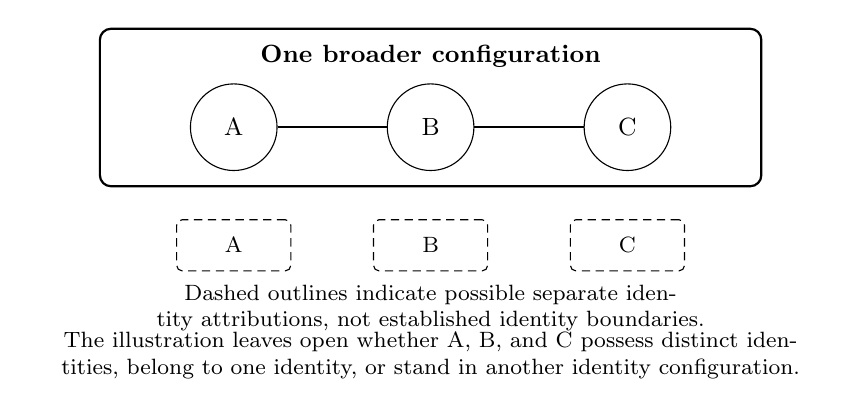
\begin{tikzpicture}[
    element/.style={
        circle,
        draw,
        minimum size=11mm,
        font=\small
    },
    possible/.style={
        draw,
        densely dashed,
        rounded corners=2pt,
        minimum width=1.45cm,
        minimum height=0.65cm,
        font=\footnotesize
    }
]

% Broader configuration
\draw[thick, rounded corners=4pt]
    (-4.2,1.0) rectangle (4.2,-1.0);

\node[font=\small\bfseries] at (0,0.65) {
    One broader configuration
};

% Elements within the configuration
\node[element] (a) at (-2.5,-0.25) {A};
\node[element] (b) at (0,-0.25) {B};
\node[element] (c) at (2.5,-0.25) {C};

\draw[thick] (a) -- (b);
\draw[thick] (b) -- (c);

% Possible identity attributions
\node[possible] at (-2.5,-1.75) {
    A
};

\node[possible] at (0,-1.75) {
    B
};

\node[possible] at (2.5,-1.75) {
    C
};

\node[
    align=center,
    text width=10cm,
    font=\footnotesize
] at (0,-2.55) {
    Dashed outlines indicate possible separate identity
    attributions, not established identity boundaries.
};

\node[
    align=center,
    text width=10cm,
    font=\footnotesize
] at (0,-3.15) {
    The illustration leaves open whether A, B, and C
    possess distinct identities, belong to one identity,
    or stand in another identity configuration.
};

\end{tikzpicture}

\caption{A unified configuration with identity attributions left open}
\label{fig:multiple-identity-attributions-within-one-configuration}

\end{figure}

% =============================================================================
% END OF ASSET IL01
% =============================================================================

The illustration provides a concrete way to consider
different possible attributions within one organized
configuration. It is illustrative rather than evidential:
it does not establish that the depicted elements possess
distinct identities, nor that the encompassing configuration
constitutes an additional identity. Those conclusions
would require independent ontological grounds.

% -----------------------------------------------------------------------------
\subsection{Plurality Without Premature Enumeration}

Even where identity plurality is established in a particular
case, its numerical structure requires further examination.
The recognition that more than one identity is involved
does not by itself determine the total number of identities,
their relations, or the principles by which they are
distinguished.

The identities involved need not be assumed to form
a collection of independent and mutually isolated units.
They may be related in ways that affect their constitution,
manifestation, or organization without necessarily
eliminating their distinction.

Likewise, the recognition of a broader configuration
does not automatically establish an additional identity
above or beyond the identities already distinguished.
A higher-order identity, if proposed, would require
its own ontological justification rather than being
inferred from the mere existence of a grouping or
composition.

For these reasons, identity plurality should not be
reduced to a numerical inventory made before the relevant
identity criteria have been clarified. Enumeration
presupposes that the units to be counted have already
been identified as identities. Where that prior
determination remains unsettled, a numerical conclusion
would merely restate the unresolved question.

% -----------------------------------------------------------------------------
\subsection{Conditions for a Responsible Attribution of Identity Plurality}

The preceding analysis indicates that an attribution
of identity plurality requires more than the observation
of multiplicity. At a minimum, an adequate account
must clarify the subject of the attribution, the respect
under which plurality is asserted, and the grounds
for distinguishing the identities involved.

It must also distinguish identity plurality from
manifestational, compositional, and relational multiplicity.
Where a common source or unified aggregate is relevant,
the account must explain precisely what follows from
that relation and what does not.

The requirements may be stated as follows:

\begin{enumerate}
    \item The entities or configurations to which identity
    is attributed must be specified.
    \item The respect and scope of the plurality claim
    must be made explicit.
    \item The grounds for distinguishing identities must
    be stated rather than inferred from difference alone.
    \item Relations among the identities must be examined
    without presuming that relation either eliminates
    or guarantees distinction.
    \item The attribution must not depend solely on the
    number of manifestations, components, relations,
    sources, or aggregates.
    \item The conclusion must remain proportionate to
    the grounds actually established.
\end{enumerate}

These requirements are methodological constraints on
ontological argument. They do not constitute a completed
definition of identity plurality, nor do they provide
a universal test that can be applied without regard
to the particular ontological problem.

Their function is to prevent unsupported transitions
from one kind of multiplicity to another and to make
explicit what an argument for identity plurality would
need to establish.

% -----------------------------------------------------------------------------
\subsection{Conclusion: Identity Plurality as an Open Ontological Problem}

Plurality of identities is a genuine ontological possibility
that cannot be excluded merely by appealing to the unity
of an existent, a common source, or a unified aggregate.
At the same time, it cannot be established merely by
counting components, manifestations, relations, or
differences between configurations.

The inquiry has therefore maintained the distinction
between identity plurality and other forms of multiplicity.
It has also shown that identity distinction requires
grounds that are relevant to identity itself. Similarity,
difference, spatial separation, material continuity,
structural integration, and relational connection may
be relevant to the analysis, but none independently
settles the question in every case.

No universal conclusion has been established here
that every existent possesses exactly one identity.
Nor has the universal attribution of multiple identities
been established. The number and organization of identities
must remain open wherever the relevant ontological
grounds have not been sufficiently determined.

The next section examines plurality and composition
more directly. It will consider the relation between
compositional organization and identity without assuming
that the plurality of components either entails or
excludes plurality of identities.

% =============================================================================
% END OF SECTION 04 OF CHAPTER 03
% =============================================================================

% ------------------------------------------------------------
% SECTION 05
% ------------------------------------------------------------

% =============================================================================
% Project : THE_PHILOSOPHY_OF_VIABILITY
% Book    : Book I — Ontology of Viability
% Book ID : VS.B01
%
% File    : 2_MAINMATTER/PART_I_IDENTITY_AND_MANIFESTATION/
%           CHAPTER_03_UNITY_AND_PLURALITY/sections/
%           section_05_plurality_and_composition.tex
%
% Section : Chapter 03, Section 05
% Title   : Plurality and Composition
%
% Purpose :
%   To examine the ontological relation between components,
%   compositional organization, wholes, and identity without
%   reducing identity to composition or inferring identity
%   plurality from component multiplicity.
%
% =============================================================================

\section{Plurality and Composition}
\label{sec:plurality-and-composition}

% -----------------------------------------------------------------------------
\subsection{The Ontological Problem of Composition}

Composition introduces a specific problem into the analysis
of unity and plurality. An existent may involve multiple
components that participate in an organized configuration.
The components may differ in their material constitution,
structural position, relations, determinations, or modes
of manifestation.

The presence of such components raises questions about
the ontological relation between the components and the
configuration in which they participate. It also raises
the question of whether the unity of that configuration
has implications for the identity attributed to it.

These questions must not be answered by counting components
alone. A plurality of components does not establish a
plurality of identities. Equally, the organization of
several components into one composition does not establish
that the composition possesses exactly one identity.

Composition and identity therefore require distinct
analyses. Their possible relation must be investigated
without presupposing that either the components or the
composed whole provide an exhaustive foundation for identity.

% -----------------------------------------------------------------------------
\subsection{Composition as an Organized Relation}

Composition is considered here as an ontological relation
through which multiple components participate in the
constitution of a more comprehensive configuration.
It is not merely the act of considering several elements
together, nor is every collection of elements necessarily
a composition in the relevant sense.

A composition may involve relations of arrangement,
organization, integration, dependence, or constitutive
participation. The specific relations involved determine
how the components belong to the configuration and how
their organization differs from an arbitrary grouping.

The concept of composition must nevertheless be distinguished
from the concept of identity. An organized composition
may be identifiable as a configuration under a specified
description without the ontological status of its identity
being settled.

Likewise, participation in a composition does not by itself
establish that a component loses every form of ontological
distinction. The components may remain differentiated
while participating in relations that constitute the whole.

Composition must therefore be examined as a relation
among constituents. It cannot be treated, without further
argument, as a complete explanation of the identity
of the resulting configuration.

% -----------------------------------------------------------------------------
\subsection{Plurality of Components and Plurality of Identities}

The plurality of components is not sufficient to establish
the plurality of identities. An existent may involve
several components while its identity remains unified
in a particular ontological respect. This possibility
blocks a direct inference from compositional multiplicity
to identity plurality.

The distinction can be expressed as follows:

\[
\text{Plurality of Components}
\not\Rightarrow
\text{Plurality of Identities}
\]

This expression does not establish that every composition
possesses one identity. It establishes only that the
number of components cannot serve as a direct measure
of the number of identities involved.

A component may participate in a composition without
being established as an independently distinct identity.
Conversely, a component may possess an identity that is
not reducible to its participation in the broader composition.
Whether either possibility obtains in a particular case
requires an independent ontological account.

The relation between components and identities must
therefore be examined without assuming a necessary
one-to-one correspondence.

% =============================================================================
% Project : THE_PHILOSOPHY_OF_VIABILITY
% Book    : Book I — Ontology of Viability
% Book ID : VS.B01
%
% File    : 4_ASSETS/tables/
%           VS.B01.P01.C03.S05.SS03.P012.TL01.components_composition_whole_and_identity.tex
%
% Asset   : TL01 — Components, Composition, Whole, and Identity
%
% Purpose :
%   To distinguish the principal ontological terms involved
%   in compositional analysis and to prevent unsupported
%   inferences from component multiplicity to identity.
%
% =============================================================================

\begin{table}[htbp]
\centering
\caption{Components, Composition, Whole, and Identity}
\label{tab:components-composition-whole-and-identity}

\small
\renewcommand{\arraystretch}{1.35}

\begin{tabular}{p{0.19\textwidth} p{0.34\textwidth} p{0.35\textwidth}}
\hline
\textbf{Term}
&
\textbf{Primary concern}
&
\textbf{What it does not establish by itself}
\\
\hline

Component
&
An element participating in a broader configuration.
&
That it possesses an independently distinct identity.
\\

Composition
&
The organized relations through which components
participate in a configuration.
&
That the resulting configuration possesses exactly
one identity.
\\

Aggregate
&
A plurality of elements considered together under
a grouping or unity criterion.
&
That the grouping constitutes a composition or
a distinct identity.
\\

Composed whole
&
A configuration considered through the organization
of its participating components.
&
That its identity is reducible to its components
or their arrangement.
\\

Structural organization
&
The positions and relations through which components
are organized.
&
That structural unity is equivalent to identity unity.
\\

Material constitution
&
The material elements and conditions involved
in the constitution of an existent.
&
That material continuity or integration determines
identity.
\\

Identity
&
The ontological unity or distinction attributable
at the level of identity.
&
That its status can be inferred solely from
component count or compositional organization.
\\

\hline
\end{tabular}

\end{table}

% =============================================================================
% END OF ASSET TL01
% =============================================================================

The table distinguishes the principal terms involved
in compositional analysis. It is not intended as an
exhaustive taxonomy. Its purpose is to prevent a conclusion
about identity from being inferred directly from a
description of components or their organization.

% -----------------------------------------------------------------------------
\subsection{Unity of Composition and Unity of Identity}

The unity of a composition does not automatically
establish the unity of identity. A composition may
exhibit extensive organization, structural integration,
or coordination among its components. These conditions
may warrant treating the components as one organized
configuration under a specified compositional respect.

Nevertheless, the unity of the configuration in that
respect does not settle whether its identity is singular,
plural, or related to the identities of its constituents
in another ontological manner.

The distinction can be expressed schematically:

\[
\text{Unity of Composition}
\not\Rightarrow
\text{Unity of Identity}
\]

This does not mean that composition is irrelevant to
identity. The organization of components may contribute
to conditions under which an identity is constituted,
maintained, or manifested. Such a contribution, however,
must be established rather than assumed.

The unity of composition and the unity of identity may
coincide in a particular existent. Their possible
coincidence does not make them conceptually equivalent,
nor does it establish a universal rule connecting them.

% -----------------------------------------------------------------------------
\subsection{Components and the Composed Whole}

The relation between components and a whole cannot
be adequately described through a simple opposition
between wholly independent parts and an entirely
self-contained whole.

Components may participate in the constitution of a
whole through relations that determine their arrangement,
dependence, and mutual contribution. At the same time,
the whole may possess determinations that cannot be
attributed to each component considered in isolation.

At least four possibilities require separate consideration:

\begin{enumerate}
    \item Components may retain distinct ontological
    determinations while participating in one composition.

    \item Components may acquire or enter into further
    determinations through their relations within
    a composition.

    \item The composed whole may exhibit determinations
    that are not attributable to the isolated components
    considered separately.

    \item The relation between components and whole may
    involve forms of dependence that cannot be described
    solely through spatial inclusion or material contact.
\end{enumerate}

These possibilities do not constitute a universal theory
of composition. They indicate that the relation between
components and whole must be examined through its
specific ontological conditions.

No conclusion about identity follows from the mere
presence of any one of these relations. In particular,
the attribution of a determination to the whole does
not automatically establish an additional identity,
and the distinction of a component does not automatically
establish an independent identity.

% -----------------------------------------------------------------------------
\subsection{Composition Without Homogeneity}

The formation of a composition does not necessarily
eliminate differences among its components. Components
may remain differentiated in their material, structural,
relational, or functional determinations while participating
in an organized whole.

Compositional unity therefore need not be understood
as the reduction of components to homogeneity. A whole
may be organized through differentiated contributions,
and the differences among its components may be relevant
to the organization of the composition.

Conversely, the preservation of differences among
components does not automatically negate the unity
of the composition. Difference and compositional unity
are not mutually exclusive in every respect.

This point must not, however, be transferred without
qualification to identity. The compatibility of internal
difference with compositional unity does not prove
identity unity. Whether differentiated components
belong to one identity or involve several identities
remains a distinct question.

% -----------------------------------------------------------------------------
\subsection{Composition and Material Constitution}

Material constitution may provide important conditions
for compositional relations. An existent may be constituted
through multiple material elements whose arrangement
and interaction contribute to its structure and
manifestation.

Material composition cannot, however, be treated as
an exhaustive definition of identity. The material
constituents of an existent may change while some
relevant ontological determinations remain preserved.
Conversely, the preservation of material constituents
does not by itself establish the preservation of identity.

Material continuity, material similarity, and material
integration are therefore insufficient as universal
criteria of identity unity or plurality. Their relevance
depends on the specific ontological question being examined.

This restriction does not imply that material constitution
is ontologically irrelevant. It means that the material
conditions of an existent must be distinguished from
the identity attributed to it. The significance of
material manifestation must be preserved without
reducing identity to material composition.

% -----------------------------------------------------------------------------
\subsection{Composition and Structural Organization}

Composition may involve structural organization through
which components occupy determinate positions and
participate in relations that constitute a configuration.
Such organization may distinguish one composition
from another and may be relevant to the conditions
under which a whole is constituted.

Structural distinction does not automatically establish
identity distinction. Two compositions may differ
structurally without that difference alone determining
whether they possess distinct identities. Conversely,
structural similarity does not establish that two
compositions share one identity.

Structural integration also cannot serve as a sufficient
criterion of identity unity. The fact that components
form a highly integrated structure does not establish,
without further argument, that the resulting whole
possesses only one identity.

The relation between composition and structure must
therefore be distinguished from the relation between
composition and identity. Structural organization
may be relevant to identity, but it cannot be treated
as an exhaustive substitute for identity itself.

% =============================================================================
% Project : THE_PHILOSOPHY_OF_VIABILITY
% Book    : Book I — Ontology of Viability
% Book ID : VS.B01
%
% File    : 4_ASSETS/diagrams/
%           VS.B01.P01.C03.S05.SS08.P032.DG01.components_composition_and_identity_relations.tex
%
% Asset   : DG01 — Components, Composition, and Identity Relations
%
% Purpose :
%   To represent the distinction between component plurality,
%   compositional organization, and identity without implying
%   that any one of these necessarily entails another.
%
% Requires (preamble):
%   \usepackage{tikz}
%   \usetikzlibrary{calc, positioning, fit}
% =============================================================================

\begin{figure}[htbp]
    \centering
    \hyphenpenalty=10000 \exhyphenpenalty=10000\relax  % no hyphenation inside diagram labels

    \begin{tikzpicture}[
        font=\small,
        node distance=0.4cm,
        % --- base box ---
        box/.style={
            draw, rounded corners=3pt, align=center,
            inner sep=6pt, line width=0.7pt
        },
        % --- node roles ---
        compbox/.style={box, text width=2.6cm, minimum height=1.1cm,
                        fill=blue!8, draw=blue!55!black},
        compositionbox/.style={box, text width=6.8cm, minimum height=1.5cm,
                               fill=blue!16, draw=blue!55!black},
        identitybox/.style={box, text width=6.8cm, minimum height=1.5cm,
                            dashed, fill=gray!10, draw=black!60},
        % --- frames and labels ---
        vsgroup/.style={draw=black!45, dashed, rounded corners=5pt,
                        inner sep=8pt, line width=0.5pt},
        grouplabel/.style={font=\footnotesize\itshape, text=black!75,
                           align=left},
        legendtext/.style={font=\scriptsize},
        % --- undirected lines (no arrowheads: no entailment, no priority) ---
        vsrel/.style={draw=black!70, line width=0.8pt},
        vslink/.style={draw=black!55, dashed, line width=0.7pt}
    ]

    % ---------------------------------------------------------------
    % Components (equal rank)
    % ---------------------------------------------------------------
    \node[compbox] (b) {Component B};
    \node[compbox, left=of b]  (a) {Component A};
    \node[compbox, right=of b] (c) {Component C};

    \node[vsgroup, fit=(a)(b)(c)] (comps) {};
    \node[grouplabel, anchor=south west] at (comps.north west) {
        Component plurality
    };

    % ---------------------------------------------------------------
    % Composition and identity
    % ---------------------------------------------------------------
    \node[compositionbox, below=1.1cm of comps] (whole) {
        \textbf{Composition}\\[3pt]
        Organized relations among components
    };
    \node[identitybox, below=1.1cm of whole] (id) {
        \textbf{Identity}\\[3pt]
        Unity or plurality requires identity-level grounds
    };

    % each component participates in the composition (straight, vertical)
    \draw[vsrel] (a.south) -- (a.south |- whole.north);
    \draw[vsrel] (b.south) -- (b.south |- whole.north);
    \draw[vsrel] (c.south) -- (c.south |- whole.north);

    % possible ontological relevance (not entailment)
    \draw[vslink] (whole) -- (id);

    % ---------------------------------------------------------------
    % Legend and interpretive constraint
    % ---------------------------------------------------------------
    \node[below=0.7cm of id, legendtext] (legend) {
        \tikz[baseline=-0.5ex]\draw[vsrel] (0,0) -- (0.6,0);~participation in an organized configuration
        \quad\quad
        \tikz[baseline=-0.5ex]\draw[vslink] (0,0) -- (0.6,0);~possible ontological relevance
    };

    \node[below=0.4cm of legend, text width=10.5cm, align=center,
          font=\footnotesize\itshape] {
        \textbf{Interpretive constraint:}
        The component-to-composition connections represent
        participation in an organized configuration. The
        composition-to-identity connection represents possible
        ontological relevance, not entailment. Component count
        and compositional unity do not determine identity number.
    };

    \end{tikzpicture}

    \caption{The distinct relations among components, composition, and identity}
    \label{fig:components-composition-and-identity-relations}
\end{figure}

% =============================================================================
% END OF ASSET DG01
% =============================================================================


The diagram distinguishes the relations among components,
composition, and identity. Its connections indicate
possible ontological relevance, not necessary entailment
or a fixed sequence of constitution.

% -----------------------------------------------------------------------------
\subsection{The Possibility of Multiple Identities Within a Composition}

The unity of a composition does not exclude the possibility
that multiple identities may be involved within it.
An organized whole may include components or subsystems
whose identity relations require independent examination.

However, the presence of differentiated components
or subsystems does not automatically establish that
each possesses a distinct identity. Such an attribution
requires grounds relevant to identity itself rather than
an inference from structural or functional differentiation.

A composition may therefore involve several determinations
at once: unity of composition, plurality of components,
differentiation of structural relations, and a possible
unity or plurality of identities. These determinations
concern different ontological respects and are not
contradictory merely because they coexist.

The possibility of multiple identities within a composition
must remain open. It must not be treated as an automatic
consequence of compositional multiplicity, nor excluded
by appealing to the unity of the composed whole.

% -----------------------------------------------------------------------------
\subsection{One Identity Across Compositional Transformation}

The relation between composition and identity also raises
the question of whether one identity may be associated
with different compositional configurations.

A composition may undergo changes in its components,
their arrangement, or their relations. Such changes
do not automatically establish the emergence of a new
identity. Nor does the preservation of a particular
composition automatically establish that the same
identity persists.

A reduction of identity to composition would tend to
treat every identity-relevant compositional change as
an identity change. An account that entirely separates
identity from composition, on the other hand, would
risk ignoring the possible constitutive significance
of compositional conditions.

Neither position can be accepted without further argument.
The relation must be examined in terms of the specific
conditions under which composition contributes to
identity constitution, manifestation, or distinction.

This inquiry must also distinguish compositional
transformation from identity persistence. The former
describes a change in the organization or constituents
of a composition; the latter concerns whether an identity
continues to obtain. One cannot be used as a substitute
for the other.

% -----------------------------------------------------------------------------
\subsection{Composition, Aggregate, and Identity}

Composition, aggregate, and identity must remain
conceptually distinct. An aggregate concerns a plurality
of elements considered together under some grouping
or unity criterion. A composition concerns relations
through which components participate in an organized
configuration. Identity concerns the ontological unity
or distinction attributable at the level of identity.

These concepts may refer to related aspects of an
existent, but they answer different questions. The
distinction can be summarized as follows:

\[
\begin{aligned}
\text{Aggregate} &\neq \text{Composition}
\\
\text{Composition} &\neq \text{Identity}
\\
\text{Unity of Composition} &\neq \text{Unity of Identity}
\\
\text{Plurality of Components} &\neq
\text{Plurality of Identities}
\end{aligned}
\]

The distinction between aggregate and composition
does not imply that every aggregate is wholly unorganized
or that every composition possesses a particular degree
of integration. It indicates that the relations through
which a whole is constituted must be specified before
conclusions about its ontological unity are drawn.

Similarly, the distinction between composition and
identity does not imply that identity is independent
of every compositional condition. It prevents composition
from being treated as sufficient, by itself, to determine
identity.

% -----------------------------------------------------------------------------
\subsection{The Limits of Compositional Reduction}

Compositional reduction occurs when identity is explained
entirely through components and their organization.
Such an account may provide important information
about the constitution of an existent, but it risks
assuming that a complete description of composition
is equivalent to a complete account of identity.

A description of components and their relations may
explain how a configuration is organized without
settling the ontological question of what identity
belongs to that configuration. The identification
of a composition is not yet an explanation of the
identity attributed to it.

The opposite reduction must also be avoided. Treating
identity as wholly independent of composition would
be premature where compositional conditions may
contribute to identity constitution, manifestation,
or distinction.

The appropriate position is therefore neither to
identify identity with composition nor to deny every
ontological relevance of composition. Composition
may be one dimension of the conditions relevant to
identity. Whether it constitutes, constrains, or
merely accompanies a particular identity relation
must be established through further analysis.

% -----------------------------------------------------------------------------
\subsection{Illustrative Case: Components and an Organized Configuration}

Consider a device assembled from several components.
The components may be distinguishable, replaceable,
or organized in different ways. Their arrangement
may constitute a functioning configuration, but the
mere fact that they form one assembled device does
not settle every question concerning identity.

The components may be considered individually, the
assembled configuration may be considered as a whole,
and the relations among the components may be examined
as a compositional organization. These are different
objects of analysis, even when they concern the same
concrete case.

% =============================================================================
% Project : THE_PHILOSOPHY_OF_VIABILITY
% Book    : Book I — Ontology of Viability
% Book ID : VS.B01
%
% File    : 4_ASSETS/illustrations/
%           VS.B01.P01.C03.S05.SS13.P047.IL01.components_and_composed_configuration.tex
%
% Asset   : IL01 — Components and Composed Configuration
%
% Purpose :
%   To illustrate the difference between distinguishable
%   components and their organization as a composed whole,
%   while leaving identity attribution unresolved.
%
% =============================================================================

\begin{figure}[htbp]
\centering

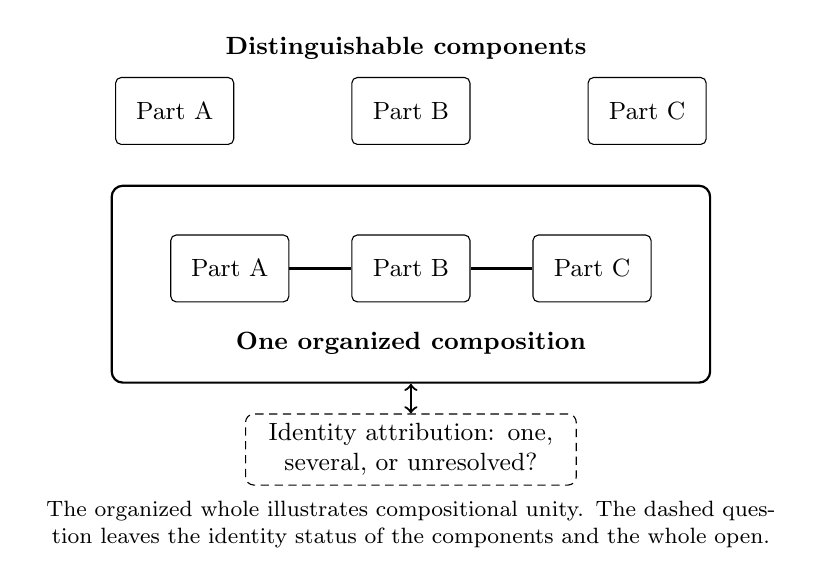
\begin{tikzpicture}[
    part/.style={
        draw,
        rounded corners=2pt,
        minimum width=1.5cm,
        minimum height=0.85cm,
        align=center,
        font=\small
    },
    whole/.style={
        draw,
        rounded corners=4pt,
        thick,
        minimum width=7.6cm,
        minimum height=2.5cm
    },
    question/.style={
        draw,
        densely dashed,
        rounded corners=3pt,
        minimum width=4.2cm,
        minimum height=0.9cm,
        align=center,
        text width=3.9cm,
        font=\small
    }
]

% Components considered separately
\node[part] (p1) at (-3.0,1.2) {Part A};
\node[part] (p2) at (0,1.2) {Part B};
\node[part] (p3) at (3.0,1.2) {Part C};

\node[align=center, font=\small\bfseries] at (0,2.0) {
    Distinguishable components
};

% Composed configuration
\node[whole] (frame) at (0,-1.0) {};

\node[part] (a) at (-2.3,-0.8) {Part A};
\node[part] (b) at (0,-0.8) {Part B};
\node[part] (c) at (2.3,-0.8) {Part C};

\draw[thick] (a) -- (b);
\draw[thick] (b) -- (c);

\node[font=\small\bfseries] at (0,-1.75) {
    One organized composition
};

% Identity question
\node[question] (identity) at (0,-3.1) {
    Identity attribution:
    one, several, or unresolved?
};

\draw[<->, thick] (frame.south) -- (identity.north);

\node[
    align=center,
    text width=9.5cm,
    font=\footnotesize
] at (0,-4.05) {
    The organized whole illustrates compositional unity.
    The dashed question leaves the identity status of
    the components and the whole open.
};

\end{tikzpicture}

\caption{Distinguishable components organized within one composition}
\label{fig:components-and-composed-configuration}

\end{figure}

% =============================================================================
% END OF ASSET IL01
% =============================================================================

The illustration is intended to clarify the distinction
between component multiplicity and compositional unity.
It does not establish whether the components or the
assembled configuration possess distinct identities.
Nor does it establish that the assembled whole constitutes
an additional identity. Those conclusions require
independent ontological grounds.

% -----------------------------------------------------------------------------
\subsection{The Relation to Unity and Plurality}

The analysis of composition clarifies that unity and
plurality cannot be attributed to an existent without
specifying their subject and respect. A composition
may be unified with respect to its organization while
remaining plural with respect to its components.

The same configuration may also raise questions of
identity unity or plurality that are not settled by
either of those descriptions. The unity of composition
and the plurality of components may coexist without
contradiction because they concern different
ontological determinations.

The relevant distinctions include:

\begin{itemize}
    \item Unity of composition and plurality of components.
    \item Unity of an aggregate and plurality of its constituents.
    \item Unity of identity and plurality of determinations.
    \item Unity of a broader configuration and possible
    plurality of identities.
\end{itemize}

These relations must not be collapsed into a single
opposition between the one and the many. The question
is not simply whether an existent is one or many. It
is necessary to determine what is one, what is many,
and whether the relevant claims concern components,
composition, aggregate, manifestation, or identity.

% -----------------------------------------------------------------------------
\subsection{Conclusion: Composition as Relevant but Non-Exclusive}

Composition is an important ontological dimension
in the examination of unity and plurality. It concerns
the relations through which multiple components
participate in an organized configuration.

Neither the plurality of components nor the unity
of their composition is sufficient, by itself, to
establish the plurality or unity of identity. Composition
may contribute to the conditions under which identity
is constituted or manifested, but it cannot be treated
as the exclusive foundation of identity.

Likewise, identity cannot be considered independent
of every compositional condition without further
argument. The ontological relation between composition
and identity must therefore be examined without
reducing either to the other.

The next section turns to the broader relation between
identity and multiplicity. It considers the different
forms of multiplicity that may occur within an existent
or across a plurality of existents, and examines why
multiplicity cannot be treated as synonymous with
plurality of identities.

% =============================================================================
% END OF SECTION 05 OF CHAPTER 03
% =============================================================================

% ------------------------------------------------------------
% SECTION 06
% ------------------------------------------------------------

% =============================================================================
% Section 06 — Identity and Multiplicity
% Book I — Ontology of Viability
% Chapter 03 — Unity and Plurality
%
% Purpose:
%   To distinguish multiplicity in its general ontological
%   sense from plurality of identities, and to examine
%   the different forms of multiplicity that may occur
%   within and across existents.
%
% Conceptual Policy:
%   1. Multiplicity is broader than plurality of identities.
%   2. Multiplicity of determinations, manifestations,
%      components, or relations does not automatically
%      establish identity plurality.
%   3. Unity of identity does not require the elimination
%      of every form of multiplicity.
%   4. Identity must not be reduced to a numerical count
%      of multiple elements.
%   5. The ontological subject and respect of every
%      multiplicity claim must be specified.
%   6. Neither universal identity unity nor universal
%      identity plurality is presupposed.
%
% =============================================================================

\section{Identity and Multiplicity}
\label{sec:identity-and-multiplicity}

% -----------------------------------------------------------------------------
\subsection{The Ontological Problem of Multiplicity}

Multiplicity is a broad ontological determination
that may occur in different forms and at different
levels of an existent or a configuration of existents.

An existent may involve multiple determinations,
components, relations, manifestations, processes,
or compositional elements.

A plurality of existents may also participate
in a broader configuration in which their relations
produce further forms of multiplicity.

However, the recognition of multiplicity does not
by itself settle the question of identity.

Multiplicity and plurality of identities are
not equivalent concepts.

The former concerns the presence of more than
one element, determination, or relation in
a specified ontological respect.

The latter concerns the existence of more than
one identity.

The distinction is essential because multiplicity
may occur without identity plurality being
established.

Conversely, identity plurality may involve
relations and forms of organization that cannot
be adequately described through a simple
enumeration of elements.

The present section examines this distinction
and establishes the conceptual conditions
necessary for discussing multiplicity without
reducing identity to it.

% -----------------------------------------------------------------------------
\subsection{Multiplicity as a General Ontological Determination}

Multiplicity refers to the presence or constitution
of more than one element, determination, relation,
or manifestation within a specified ontological
domain or respect.

Its meaning depends on what is being considered
multiple.

Multiplicity may concern:

\begin{itemize}
    \item Components of an existent.
    \item Determinations belonging to an existent.
    \item Relations in which an existent participates.
    \item Manifestations associated with an existent.
    \item Processes or transformations involving
    an existent.
    \item Existents participating in a broader
    configuration.
\end{itemize}

These forms of multiplicity are not identical.

A plurality of components concerns compositional
multiplicity.

A plurality of determinations concerns the
differentiation of what characterizes an existent.

A plurality of relations concerns the multiplicity
of relational connections.

A plurality of manifestations concerns the
multiplicity of ways in which an existent
is manifested.

Each form requires its own ontological analysis.

The general concept of multiplicity therefore
cannot be treated as a single undifferentiated
category.

More importantly, none of these forms can
automatically be transferred into a conclusion
about the number of identities involved.

% -----------------------------------------------------------------------------
\subsection{Multiplicity and the Subject of Multiplicity}

Every claim of multiplicity requires the
identification of its subject.

To say that something is multiple is incomplete
unless it is specified what is being considered
multiple.

The subject may be an existent, a composition,
a set of determinations, a relational configuration,
a manifestation, or identity itself.

These subjects cannot be treated as interchangeable.

For example, an existent may be multiple in
its components while unified in another respect.

It may also exhibit several manifestations
without the identity relation among those
manifestations being determined.

Similarly, a plurality of existents may form
one aggregate without thereby constituting
one identity.

The subject of multiplicity must therefore
be distinguished from the subject of identity.

This requirement prevents the transfer of
a numerical description from one ontological
domain to another without justification.

A multiplicity claim must consequently specify:

\begin{enumerate}
    \item What is considered multiple.
    \item The domain in which multiplicity occurs.
    \item The ontological respect under consideration.
    \item The relation, if any, between that
    multiplicity and identity.
\end{enumerate}

Without these distinctions, the term multiplicity
risks becoming too broad to support precise
ontological conclusions.

% -----------------------------------------------------------------------------
\subsection{Multiplicity Does Not Necessarily Imply Identity Plurality}

The central distinction of this section is that
multiplicity does not necessarily imply plurality
of identities.

An existent may involve numerous components,
determinations, relations, or manifestations
without this multiplicity automatically
establishing more than one identity.

The relation can be expressed as follows:

\[
\text{Multiplicity}
\not\Rightarrow
\text{Plurality of Identities}
\]

This expression does not establish that
multiplicity and identity plurality are
unrelated.

It establishes that the former is not
a sufficient condition for the latter.

The presence of multiple elements may be
relevant to an investigation of identity,
but the ontological significance of those
elements must be independently demonstrated.

For example, the plurality of components
within a composition does not by itself
establish that each component possesses
a distinct identity.

Likewise, the plurality of manifestations
associated with an existent does not
establish that each manifestation constitutes
a separate identity.

The inference from multiplicity to identity
plurality therefore requires an additional
account of identity distinction.

Without such an account, the inference
remains unsupported.

% -----------------------------------------------------------------------------
\subsection{Identity Unity Does Not Require the Elimination of Multiplicity}

The distinction must also be maintained
in the opposite direction.

The unity of identity does not necessarily
require the absence of multiplicity.

An existent may involve multiple determinations,
components, relations, or manifestations
while its identity remains unified in
a particular ontological respect.

Unity of identity therefore cannot be defined
simply as the elimination of multiplicity.

Such a definition would confuse unity with
homogeneity or numerical indivisibility.

It would also impose an unnecessary opposition
between identity unity and internal differentiation.

The presence of multiplicity may be compatible
with unity, but this compatibility does not
mean that every multiplicity is necessarily
contained within one identity.

The relevant question is whether the multiplicity
under consideration belongs to the constitution,
manifestation, or relations of one identity,
or whether it involves a plurality of identities.

That question cannot be settled by the mere
recognition of multiplicity.

The distinction must be established through
an examination of the ontological subject
and the relations involved.

% -----------------------------------------------------------------------------
\subsection{Multiplicity of Determinations}

An existent may possess multiple determinations
that distinguish different aspects of its
ontological constitution.

These determinations may concern different
domains, relations, modes, or conditions
of existence.

Their plurality does not automatically imply
that the existent possesses multiple identities.

A plurality of determinations may be compatible
with the unity of identity.

However, this possibility must not be turned
into the assumption that all determinations
necessarily belong to one identity.

The relation between determinations and identity
requires an account of how determinations
participate in the constitution or distinction
of identity.

A determination may be relevant to identity
without being identical to identity.

Likewise, the plurality of determinations
may contribute to the differentiation of
an existent without establishing identity
plurality.

The distinction between identity and its
determinations must therefore be preserved.

This also prevents identity from being reduced
to a list or aggregate of features.

An inventory of determinations may describe
an existent, but it does not by itself
provide an exhaustive account of its identity.

% -----------------------------------------------------------------------------
\subsection{Multiplicity of Manifestations}

Multiplicity may also occur at the level
of manifestation.

An existent may manifest through different
configurations, forms, or modes.

These manifestations may be related to
one another in different ways.

They may exhibit continuity, transformation,
difference, or other forms of ontological
relation.

However, the multiplicity of manifestations
does not automatically determine whether
one identity or multiple identities are involved.

A plurality of manifestations may be associated
with one identity, but this cannot be assumed
as a universal rule.

Likewise, distinct manifestations may involve
distinct identities, but their difference
does not establish that conclusion by itself.

The relation between manifestation and identity
must therefore be examined without imposing
a direct numerical correspondence.

This distinction is particularly important
when an existent undergoes transformation.

A change in manifestation does not automatically
establish a change in identity.

Nor does the preservation of a recognizable
manifestational configuration automatically
establish identity continuity.

The relevant ontological relations require
independent analysis.

% -----------------------------------------------------------------------------
\subsection{Multiplicity of Relations}

An existent may participate in multiple
relations with other existents or with
different ontological domains.

These relations may differ in their nature,
scope, direction, or significance.

Relational multiplicity does not automatically
establish plurality of identities.

One identity may be involved in multiple
relations without thereby becoming multiple.

Conversely, the unity of a relational subject
does not automatically exclude the possibility
that a broader configuration involves
multiple identities.

The number of relations and the number
of identities therefore concern different
ontological questions.

A relational configuration may also involve
relations among several identities, but
this possibility must be established through
the ontological distinction of the related
subjects.

It cannot be inferred merely from the
multiplicity of relational connections.

The analysis must therefore distinguish
relational multiplicity from identity plurality
while preserving the possibility that
relations may be relevant to identity
constitution and distinction.

% -----------------------------------------------------------------------------
\subsection{Multiplicity of Processes and Transformations}

Multiplicity may also concern processes
and transformations.

An existent may undergo several transformations
or participate in multiple processes
throughout its existence.

Such multiplicity may involve changes
in determinations, structure, composition,
relations, or manifestation.

However, the plurality of transformations
does not automatically establish plurality
of identities.

Nor does the existence of multiple processes
necessarily indicate that one identity
is involved.

A process may be associated with one identity,
with several identities, or with a configuration
whose identity relations remain undetermined.

The ontological status of the process and
the identity of the existent must therefore
be examined separately.

This distinction also prevents the reduction
of identity to a sequence of states or events.

A temporal or processual description may
provide relevant information about an existent,
but it does not by itself settle the question
of identity unity or plurality.

% -----------------------------------------------------------------------------
\subsection{Multiplicity Across Different Ontological Respects}

Multiplicity may be present in one ontological
respect while unity is present in another.

An existent may be materially composite,
structurally organized, relationally differentiated,
and unified in some other respect.

These descriptions need not contradict one another
because they concern different determinations.

The same applies to plurality of existents.

Several existents may constitute one aggregate
in a compositional respect while remaining
distinct in their identities.

Likewise, multiple manifestations may be
related through one source without their
identity relations being settled.

The distinction between different respects
prevents unity and plurality from being
treated as mutually exclusive descriptions
in every case.

The ontological question must instead determine
whether the relevant claims concern the same
subject and the same respect.

Only when they concern the same subject
under the same respect does an apparent
opposition require further resolution.

The following schematic expressions illustrate
the distinction:

\[
\begin{aligned}
&\text{Unity of Identity}
\quad+\quad
\text{Multiplicity of Determinations}
\\[4pt]
&\text{Unity of Composition}
\quad+\quad
\text{Multiplicity of Components}
\\[4pt]
&\text{Unity of Source}
\quad+\quad
\text{Multiplicity of Manifestations}
\end{aligned}
\]

These expressions indicate possible combinations
of unity and multiplicity across different
ontological respects.

They do not establish that every such combination
necessarily occurs in every existent.

% -----------------------------------------------------------------------------
\subsection{Multiplicity and the Problem of Ontological Levels}

The examination of multiplicity also requires
attention to the ontological level at which
a plurality is attributed.

A plurality may concern elements within
an existent, relations among existents,
or a broader configuration in which multiple
existents participate.

These levels must not be collapsed.

For example, the multiplicity of components
within one composition is not equivalent
to the plurality of existents participating
in a larger configuration.

Likewise, the plurality of existents within
a configuration does not automatically
establish plurality of identities at every
level of that configuration.

The ontological relation between levels
requires separate analysis.

A broader whole may involve relations among
multiple existents without necessarily
constituting a new identity.

Conversely, the possibility of a broader
identity cannot be rejected merely because
the whole contains multiple existents.

The relation between levels of organization
and identity therefore remains an open
ontological problem.

It cannot be resolved by assuming that
identity is always located at the level
of the smallest component or the largest
configuration.

% -----------------------------------------------------------------------------
\subsection{Multiplicity and Numerical Enumeration}

Numerical enumeration may be useful for
describing multiplicity.

It may establish that a specified domain
contains several components, manifestations,
relations, or existents.

However, numerical enumeration alone
does not establish the ontological nature
of the entities being counted.

Counting components does not determine
the number of identities.

Counting manifestations does not determine
the number of identities.

Counting relations does not determine
the number of identities.

The numerical result depends on the
ontological classification of what is
being counted.

If the counted elements are components,
the result concerns component plurality.

If they are manifestations, the result
concerns manifestational plurality.

If they are identities, the result concerns
identity plurality.

The category of enumeration must therefore
be established before numerical conclusions
are transferred to identity.

This prevents the use of numerical unity
or plurality as a substitute for ontological
analysis.

% -----------------------------------------------------------------------------
\subsection{The Relation Between Multiplicity and Difference}

Multiplicity is related to difference,
but the two concepts are not identical.

Multiplicity concerns the presence of more
than one element or determination in
a specified respect.

Difference concerns the distinction between
determinations, elements, or entities.

A plurality may include elements that are
similar in some respects and different
in others.

Likewise, difference may occur within
one existent without establishing plurality
of identities.

The presence of difference therefore does
not automatically establish identity plurality.

Conversely, the existence of multiple identities
does not require that they differ in every
possible determination.

Distinct identities may share determinations
or exhibit similarities without thereby
becoming one identity.

The relation between difference and identity
must therefore be examined independently
of numerical multiplicity.

This distinction is necessary to prevent
both the reduction of identity to similarity
and the reduction of plurality to difference
of appearance.

% -----------------------------------------------------------------------------
\subsection{The Limits of Multiplicity-Based Explanations of Identity}

Multiplicity-based explanations of identity
risk treating the number or arrangement
of elements as sufficient to determine
the identity of an existent.

Such explanations may describe important
features of composition, manifestation,
or relational organization.

However, they do not necessarily explain
why a particular identity is ontologically
unified or distinct.

A complete account of identity cannot
be replaced by an inventory of multiple
determinations.

Nor can identity plurality be established
by merely identifying several components
or manifestations.

The analysis must explain the ontological
relation between multiplicity and identity.

This requires a distinction between:

\begin{enumerate}
    \item Multiplicity as a condition or
    determination of an existent.

    \item Identity as an ontological
    determination of that existent.

    \item Plurality as a possible relation
    among identities.

    \item The relations through which
    multiplicity and identity may be connected.
\end{enumerate}

These distinctions do not imply that identity
and multiplicity are unrelated.

They prevent the assumption that one can
be fully explained through the other.

% -----------------------------------------------------------------------------
\subsection{Conclusion: Multiplicity Does Not Decide Identity}

Multiplicity is a broad ontological
determination that may occur in components,
determinations, relations, manifestations,
processes, and configurations.

Plurality of identities is a more specific
ontological claim concerning the existence
of more than one identity.

The two concepts must therefore remain distinct.

Multiplicity does not automatically establish
identity plurality.

Likewise, unity of identity does not require
the elimination of every form of multiplicity.

Unity and multiplicity may coexist when
they concern different ontological respects,
but their relation must be examined rather
than assumed.

The central methodological requirement
is to specify the subject, domain, and
respect of every claim of unity or plurality.

The next section examines the non-equivalence
of unity and singularity.

It considers why unity cannot be reduced
to numerical oneness and why numerical
singularity cannot serve as a complete
ontological explanation of identity.

% =============================================================================
% End of Section 06
% =============================================================================

% ------------------------------------------------------------
% SECTION 07
% ------------------------------------------------------------

% =============================================================================
% Section 07 — Non-Equivalence of Unity and Singularity
% Book I — Ontology of Viability
% Chapter 03 — Unity and Plurality
%
% Purpose:
%   To establish the ontological distinction between unity
%   and numerical singularity, and to examine why neither
%   concept can be reduced to the other.
%
% Conceptual Policy:
%   1. Unity is not equivalent to numerical singularity.
%   2. Numerical oneness does not establish unity of identity.
%   3. Unity does not necessarily imply the existence
%      of exactly one identity.
%   4. Plurality does not necessarily negate unity.
%   5. Unity must not be reduced to indivisibility,
%      homogeneity, or numerical oneness.
%   6. No universal conclusion concerning the number
%      of identities is adopted.
%
% =============================================================================

\section{Non-Equivalence of Unity and Singularity}
\label{sec:non-equivalence-of-unity-and-singularity}

% -----------------------------------------------------------------------------
\subsection{The Problem of Equating Unity with Singularity}

Unity and singularity are frequently treated as
equivalent determinations.

When something is described as one, it may be assumed
that it is singular in every relevant ontological
respect. Conversely, when something is described
as multiple, it may be assumed that unity is absent.

Such assumptions introduce a conceptual reduction
that must be examined.

Unity concerns the ontological determination through
which something is considered unified in a specified
respect.

Singularity, in its numerical sense, concerns
the condition of being one rather than more than
one within a particular domain of enumeration.

These concepts may coincide in particular cases,
but their possible coincidence does not establish
their equivalence.

The question is therefore not whether unity and
singularity can occur together.

It is whether one can be defined, established,
or inferred solely through the other.

The present section argues that such a reduction
is not ontologically justified.

% -----------------------------------------------------------------------------
\subsection{Unity as Distinct from Numerical Oneness}

Unity cannot be defined simply as numerical oneness.

Numerical oneness indicates that something is
counted as one within a specified domain and
under a particular criterion of enumeration.

Unity, however, concerns the ontological respect
in which something is considered unified.

The difference is important because numerical
counting presupposes that the subject of counting
and the criterion of individuation have already
been sufficiently determined.

It does not independently establish the ontological
unity of what is counted.

For example, an existent may be counted as one
object within a particular classification while
the unity of its identity remains an independent
ontological question.

Likewise, a system may be treated as one unit
for a particular practical or analytical purpose
without this designation establishing that
it possesses exactly one identity.

The numerical designation of one therefore
cannot replace an account of unity.

The following distinction must be maintained:

\[
\text{Numerical Oneness}
\neq
\text{Ontological Unity}
\]

This distinction does not deny that numerical
oneness may be relevant to the examination
of unity.

It denies that numerical oneness is sufficient
to establish it.

% -----------------------------------------------------------------------------
\subsection{Singularity as a Determination of Number}

Singularity concerns the numerical determination
of a subject as one within a specified domain
of counting.

Such a determination depends on what is being
counted and on the criterion through which
the counted subject is distinguished.

An existent may be considered singular as
a material object, a system, an organism,
or a bounded configuration.

However, these numerical descriptions do not
necessarily settle the question of identity.

The same existent may be singular under one
criterion of enumeration while involving
a plurality of components, relations,
or manifestations.

Likewise, several entities may be counted
as distinct units without this counting
establishing the ontological nature of their
identities.

Singularity is therefore meaningful only
in relation to a specified subject and
a specified numerical domain.

It cannot be treated as an unrestricted
ontological determination that automatically
applies to every aspect of an existent.

% -----------------------------------------------------------------------------
\subsection{The Difference Between Unity and Indivisibility}

Unity must also be distinguished from
indivisibility.

Indivisibility concerns whether something
can be divided into parts or whether such
division is possible under a specified
criterion.

Unity concerns the ontological respect
in which something is unified.

An existent may be divisible into components
while remaining unified in another respect.

Conversely, something may be treated as
indivisible within a particular analysis
without this establishing the unity of
its identity.

The possibility of division does not
automatically negate unity.

Nor does the absence of an identified
division establish unity.

The distinction can be expressed as follows:

\[
\text{Divisibility}
\not\Rightarrow
\text{Absence of Unity}
\]

and

\[
\text{Indivisibility}
\not\Rightarrow
\text{Unity of Identity}
\]

These expressions prevent the reduction
of unity to the absence of internal parts.

A theory of unity must therefore explain
the relevant ontological relation rather
than rely exclusively on criteria of
division or indivisibility.

% -----------------------------------------------------------------------------
\subsection{The Difference Between Unity and Homogeneity}

Unity is not equivalent to homogeneity.

Homogeneity concerns similarity or sameness
among elements or determinations in a
specified respect.

Unity concerns the ontological unity
attributable to a subject.

An existent may involve heterogeneous
components or differentiated determinations
while remaining unified in a relevant
ontological respect.

Likewise, several homogeneous elements
may remain distinct and may not constitute
one identity.

Similarity does not establish unity,
and difference does not necessarily negate it.

The reduction of unity to homogeneity
would impose the assumption that internal
difference is incompatible with unity.

Such an assumption is not justified.

Unity must therefore remain conceptually
distinct from the degree of similarity
among the elements or determinations
of a subject.

% -----------------------------------------------------------------------------
\subsection{The Possibility of Unity Within Plurality}

Unity and plurality are not necessarily
mutually exclusive.

A subject may be unified in one respect
while involving plurality in another.

An existent may exhibit unity of identity
while containing multiple components,
relations, or determinations.

A composition may be unified as a whole
while its constituents remain plural.

A source may be one while being related
to multiple manifestations.

These possibilities indicate that the
presence of plurality does not automatically
negate every form of unity.

However, the recognition of unity within
plurality must not be used to assume
that every plurality is necessarily
contained within one identity.

The subject and respect of each claim
must remain explicit.

The distinction can be represented
schematically:

\[
\text{Unity in one respect}
\quad+\quad
\text{Plurality in another respect}
\]

This expression indicates a possible
ontological configuration rather than
a universal rule.

It requires that the relevant respects
be distinguished before the relation
between unity and plurality is determined.

% -----------------------------------------------------------------------------
\subsection{The Possibility of Plurality Without Singular Identity}

The non-equivalence of unity and singularity
also requires that plurality not be treated
as a simple negation of every possible
form of unity.

A configuration may involve multiple
identities while exhibiting unity in
another ontological respect.

For example, several identities may participate
in one aggregate or may be related within
a broader configuration.

The unity of that aggregate or configuration
does not necessarily eliminate the distinction
among the identities involved.

Likewise, the existence of multiple identities
does not automatically establish that
they form one higher identity.

The relation between the plurality of
identities and the unity of a broader
configuration must therefore be examined
independently.

This possibility prevents the assumption
that unity can exist only where numerical
singularity is established.

% -----------------------------------------------------------------------------
\subsection{Unity and the Number of Identities}

The distinction between unity and singularity
has a direct consequence for the ontology
of identity.

The unity attributed to an existent cannot
be used, by itself, to establish that
the existent possesses exactly one identity.

Such an inference would confuse the unity
of a subject in a specified respect with
the numerical determination of its identities.

Conversely, the recognition of numerical
multiplicity within an existent does not
automatically establish that multiple
identities are involved.

The number of identities requires an
independent ontological examination.

The following implications must therefore
be rejected as automatic conclusions:

\[
\text{Unity}
\not\Rightarrow
\text{Exactly One Identity}
\]

\[
\text{Numerical Singularity}
\not\Rightarrow
\text{Unity of Identity}
\]

\[
\text{Plurality of Elements}
\not\Rightarrow
\text{Plurality of Identities}
\]

These restrictions preserve the distinction
between the ontological unity of a subject,
its numerical description, and the number
of identities involved.

They also prevent the premature adoption
of a universal doctrine of either one
identity or multiple identities.

% -----------------------------------------------------------------------------
\subsection{Unity and the Problem of the Subject}

Every attribution of unity must specify
its subject.

The statement that something is unified
remains incomplete until it is established
what is being considered unified.

The subject may be:

\begin{itemize}
    \item An existent.
    \item An identity.
    \item A source.
    \item An aggregate.
    \item A composition.
    \item A configuration of relations.
    \item A plurality of manifestations.
\end{itemize}

These subjects may be related, but their
unity cannot be assumed to be interchangeable.

The unity of an aggregate does not automatically
establish the unity of its components.

The unity of a source does not automatically
establish the unity of its manifestations.

The unity of an existent does not automatically
settle the number of identities involved.

The specification of the subject is therefore
a necessary condition for meaningful claims
about unity.

The same requirement applies to numerical
singularity.

A numerical claim is incomplete unless
the domain of enumeration and the criterion
of counting are specified.

% -----------------------------------------------------------------------------
\subsection{The Limits of Numerical Classification}

Numerical classification may be useful
for distinguishing one subject from several
subjects within a specified domain.

However, numerical classification cannot
provide a complete ontological account
of unity or identity.

Counting presupposes a criterion through
which the relevant units are identified.

That criterion may be appropriate for
a particular domain while remaining
insufficient for determining identity.

A collection may be counted as one aggregate,
a system as one functional unit, or an
existent as one material object.

None of these numerical classifications
automatically determines whether one
or multiple identities are involved.

The ontological significance of numerical
classification must therefore be established
rather than assumed.

A numerical description may contribute
to an ontological inquiry, but it cannot
replace the distinctions required by
that inquiry.

% -----------------------------------------------------------------------------
\subsection{Unity Without an Assumption of Universal Singularity}

Rejecting the equivalence between unity
and singularity does not mean rejecting
the possibility of singular identity.

An existent may possess one identity
in a particular ontological configuration.

Such a conclusion, however, requires
an argument concerning identity itself.

It cannot be established merely through
the numerical designation of one existent
or through the recognition of unity in
its composition, source, or manifestation.

Likewise, the possibility of multiple
identities must remain open where the
relevant ontological conditions support
such an examination.

The present section therefore does not
replace a universal doctrine of singularity
with a universal doctrine of plurality.

It rejects the assumption that the question
can be settled through the concept of unity
alone.

The number and relation of identities
must be examined independently.

% -----------------------------------------------------------------------------
\subsection{Conclusion: Unity and Singularity as Distinct Concepts}

Unity and singularity are distinct ontological
and numerical determinations.

Unity concerns the ontological respect
in which a subject is considered unified.

Singularity concerns its numerical
determination as one within a specified
domain of enumeration.

Neither concept can be reduced to the other.

Unity does not automatically establish
exactly one identity.

Numerical singularity does not automatically
establish unity of identity.

Divisibility, indivisibility, homogeneity,
and numerical classification likewise
cannot serve as exhaustive definitions
of unity.

The distinction also makes it possible
to recognize unity and plurality within
the same broader ontological configuration
without treating them as contradictory
in every respect.

The next section examines the limits
of unity and plurality.

It considers the conditions under which
claims of unity or plurality become
ontologically insufficient, and why
neither determination can be extended
beyond the subject and respect for which
it has been established.

% =============================================================================
% End of Section 07
% =============================================================================

% ------------------------------------------------------------
% SECTION 08
% ------------------------------------------------------------

% =============================================================================
% Project : THE_PHILOSOPHY_OF_VIABILITY
% Book    : Book I — Ontology of Viability
% Book ID : VS.B01
%
% File    : 2_MAINMATTER/PART_I_IDENTITY_AND_MANIFESTATION/CHAPTER_03_UNITY_AND_PLURALITY/sections/section_08_limits_of_unity_and_plurality.tex
%
% Section:
%   Section 08 — Limits of Unity and Plurality
%
% Purpose :
%   To establish the ontological and inferential limits of claims
%   concerning unity and plurality; distinguish what can be
%   established about a subject from what remains unresolved
%   concerning identity, source, aggregate, composition,
%   manifestation, and ontological respect; and prevent the
%   unrestricted transfer of conclusions from one determination
%   to another.
%
% Conceptual Policy:
%   1. Neither unity nor plurality is treated as a universal
%      ontological priority.
%   2. Every claim must specify its subject, respect, domain,
%      and scope.
%   3. Multiplicity does not automatically establish plurality
%      of identities.
%   4. Unity does not automatically establish singular identity.
%   5. Source, aggregate, composition, structure, manifestation,
%      and identity remain distinct ontological questions.
%   6. Numerical classification does not determine identity-number.
%   7. Conclusions must not exceed the grounds that support them.
%   8. Unresolved questions remain explicitly open.
%
% =============================================================================

\section{Limits of Unity and Plurality}
\label{sec:limits-of-unity-and-plurality}

% -----------------------------------------------------------------------------
\subsection{The Need to Establish the Limits of Unity and Plurality}

The preceding sections have examined unity and plurality
through several distinct ontological questions. They have
distinguished unity of identity from unity of source,
aggregate, and composition; examined the possibility of
plurality within a configuration; differentiated multiplicity
from plurality of identities; and rejected the equivalence
of unity with numerical singularity. These distinctions
establish a necessary conceptual basis, but they do not
by themselves determine the full scope of either unity
or plurality.

A further problem must therefore be addressed: what may
legitimately be inferred when unity or plurality has been
established, and where must the inference stop? An
ontological determination may be valid within a specified
respect without being valid in every other respect. A
claim may accurately describe the organization of a
composition while leaving the identity of that composition
unresolved. Likewise, a plurality of manifestations may
be established without determining whether the identities
involved are one or multiple.

Without explicit limits, unity and plurality can become
unrestricted explanatory principles. Unity may be invoked
to explain every form of coherence, organization, relation,
or identity, while plurality may be invoked to explain
every form of distinction, differentiation, or internal
multiplicity. Both uses exceed what these determinations
can establish on their own. The task of this section is
therefore not to diminish the ontological significance
of unity or plurality, but to delimit the conclusions
that can be drawn from them.

The limits considered here are not merely limitations
of language or classification. They concern the validity
of ontological inference. A determination established
in one respect cannot be transferred to another simply
because the same existent is involved in both claims.
The subject may remain the same while the ontological
question changes. The analysis must therefore distinguish
the subject under examination from the particular
determination attributed to it.

% -----------------------------------------------------------------------------
\subsection{The Limit of Unity as a Universal Principle}

Unity cannot be assumed to be the universal ontological
ground of every existent or every determination of an
existent. The recognition that a subject is unified in
a particular respect does not establish that all of its
determinations, components, relations, and manifestations
derive from one undifferentiated unity. Nor does it
establish that every entity related to that subject
belongs to one identity or is absorbed into one ontological
whole.

The unity attributed to a source, for example, does not
automatically determine the identity of everything related
to that source. A common source may be relevant to the
origin, constitution, or relation of several entities,
but the identity relations among those entities remain
a separate question. Similarly, the unity of an aggregate
does not establish that its components constitute one
identity. The unity of a composition may concern its
organization without settling the identity status of
the composed subject or the components involved.

A universal principle of unity would also risk treating
every plurality as merely apparent or derivative. Such
a conclusion cannot be obtained from the recognition
of unity in a particular subject. If several entities
are related within a unified configuration, their
distinctions cannot be eliminated merely by referring
to the unity of that configuration. The relation between
the unity of the broader subject and the distinctions
among its constituents requires independent examination.

Unity may therefore be ontologically significant without
being an exhaustive explanation of every relation within
or beyond its subject. Its explanatory scope must remain
limited to the respect in which it has been established.
Any extension beyond that respect requires additional
grounds identifying the relevant relation and explaining
why the original unity claim applies to the further
subject or determination.

% -----------------------------------------------------------------------------
\subsection{The Limit of Plurality as a Universal Principle}

Plurality cannot be assumed to be the universal
ontological condition of every existent. The presence
of multiple determinations, components, relations,
manifestations, or processes does not establish that
the subject consists of multiple identities. These
forms of multiplicity may be ontologically relevant,
but their relevance does not make them interchangeable
with identity plurality.

A plurality of components may belong to a composition
whose identity remains a separate question. Multiple
relations may determine or connect a subject without
each relation constituting an identity. Several
manifestations may be associated with an existent
without their number determining the number of
identities involved. In each case, the plurality
established concerns a specified kind of element,
not automatically the identity of the broader subject.

The universalization of plurality would produce an
opposite reduction to the universalization of unity.
It would treat every internal difference as evidence
of multiple identities and every differentiated
configuration as ontologically plural in the same
respect. That inference would confuse the existence
of distinctions with the ontological status of the
distinguished items. Distinction is relevant to an
analysis of plurality, but the kind and significance
of the distinction must still be established.

Plurality is therefore indispensable where multiple
subjects or elements are established within a specified
domain and respect. It cannot replace the analysis
of what is being distinguished, what kind of plurality
is involved, and whether that plurality has any
implication for identity. The transition from a
plurality of elements to a plurality of identities
requires an independent ontological argument.

% -----------------------------------------------------------------------------
\subsection{The Limit of Inferring Identity from Unity}

Unity alone cannot determine the number or structure
of identities. An existent may be described as unified
as an aggregate, a composition, a material configuration,
a relational arrangement, or a structured whole. Such
descriptions may establish unity within particular
respects, but they do not independently establish
that exactly one identity is involved.

The following inference is therefore insufficient:

\[
\text{Unity of a Subject}
\not\Rightarrow
\text{Exactly One Identity}.
\]

The insufficiency does not arise because unity is
irrelevant to identity. Unity may be relevant to an
identity-related investigation, and in some cases
a unity claim may form part of an argument concerning
identity. The problem is that the unity claim alone
does not supply the additional premises required to
determine identity-number. The subject of unity may
not be identical with the subject whose identity
is being investigated, and the respect in which
unity is established may not be the respect relevant
to identity.

To infer singular identity from unity, an account
would have to establish at least the relevant identity
subject, the grounds on which its identity is determined,
and the relation between those grounds and the unity
already established. It would also have to exclude
the possibility that the unity belongs to an aggregate,
composition, or configuration involving more than
one identity. Without such an account, the conclusion
exceeds the premises.

This restriction does not deny the possibility of
singular identity. It prevents singular identity
from being treated as an automatic consequence of
unity. The conclusion may be established in a
particular case, but it must be supported by an
argument appropriate to identity rather than inferred
from the use of the term ``one'' or from a unity
attributed to another ontological subject.

% -----------------------------------------------------------------------------
\subsection{The Limit of Inferring Identity from Plurality}

Plurality alone cannot determine the number of
identities either. The presence of several components,
relations, determinations, manifestations, or processes
does not establish that each constitutes a distinct
identity. The inference from plurality to identity
multiplicity therefore exceeds what the recognition
of plurality alone can support.

This restriction may be expressed as:

\[
\text{Plurality of Elements}
\not\Rightarrow
\text{Plurality of Identities}.
\]

The expression ``plurality of elements'' must itself
be specified. Components may be materially distinct,
relations may be numerically multiple, manifestations
may differ in form, and determinations may be
distinguishable under different respects. These
pluralities do not necessarily have the same
ontological status. Even when each plurality is
correctly established, the identity question remains:
what is the relation between the distinguished
elements and the identity or identities under
consideration?

A plurality of components may belong to one
composition, but this possibility does not establish
that every composition has one identity. Several
manifestations may be related to one existent, but
this possibility does not establish that all
manifestations in every case belong to one identity.
Multiple relations may participate in the determination
of a subject without independently establishing
multiple identities. Each example limits an inference;
none supplies a universal conclusion about identity-number.

The converse reduction must also be avoided. The
failure of plurality of elements to prove plurality
of identities does not prove that only one identity
is involved. The absence of a sufficient argument
for plurality is not a sufficient argument for unity.
The identity status of the subject must remain open
where the relevant ontological grounds have not
been established.

% -----------------------------------------------------------------------------
\subsection{The Limits of Source-Based Explanations}

The distinction between source and aggregate places
an important restriction on explanations of unity
and plurality. A source may be relevant to the
constitution, origin, or relation of multiple entities
or manifestations. However, the existence of a common
source does not automatically establish that all
related entities possess one identity. A source
relation is not, merely by being common, an identity
relation.

The plurality of manifestations also cannot be used
to infer the plurality of sources without an
independent argument. Several manifestations may
be related to one source, while a plurality of
sources may also be related to a broader configuration.
The number of manifestations and the number of
sources are distinct questions. Neither can be
determined solely by counting the other.

A source-based explanation must therefore specify
what is meant by source and what relation is being
asserted. It must distinguish origin, production,
dependence, constitution, and association wherever
these relations are relevant. These relations may
have different ontological implications. A common
origin does not necessarily imply present identity;
a relation of dependence does not necessarily imply
composition; and a shared source does not necessarily
establish a single identity among the entities
related to it.

The same restriction applies to the unity of source.
Even if a source is established as one in a particular
respect, the unity of that source cannot simply be
transferred to its manifestations or effects. The
ontological status of what is related to a source
must be examined in its own right. Source may explain
a relation, but it cannot substitute for an account
of identity.

% -----------------------------------------------------------------------------
\subsection{The Limits of Aggregate and Compositional Unity}

An aggregate may possess unity as an organized,
bounded, or related configuration. A composition
may also exhibit unity through the organization
or interrelation of its components. Such unity
may be significant for understanding the subject,
but it does not automatically establish that the
aggregate or composition constitutes one identity.

The components of an aggregate or composition may
retain distinctions that cannot be eliminated
merely by describing them as parts of one whole.
Their material, structural, relational, or other
determinations may remain relevant to their
ontological status. Conversely, the presence of
multiple components does not establish that the
aggregate lacks every form of unity. The plurality
of components and the unity of the composed
configuration may concern different respects.

The following restrictions must therefore be
maintained:

\[
\text{Unity of Composition}
\not\Rightarrow
\text{Unity of Identity}
\]

\[
\text{Plurality of Components}
\not\Rightarrow
\text{Plurality of Identities}.
\]

These restrictions prevent composition from becoming
either a universal foundation of identity or an
automatic negation of unity. They also prevent
the number of components from being treated as
a direct measure of the number of identities.

The philosophical debate concerning material
composition illustrates why the relation between
parts and wholes cannot be assumed to have one
uncontroversial solution. Different accounts
disagree about when parts compose an object and
what ontological status should be assigned to
ordinary composite entities. These debates are
relevant as comparative problems, but no particular
solution to the problem of composition is adopted
here as a premise for the ontology of identity.\footnote{For contrasting approaches to material composition and the relation between parts and wholes, see Peter van Inwagen, \textit{Material Beings} (1990), and Peter Simons, \textit{Parts: A Study in Ontology} (1987), both recorded in the bibliography of this volume.}

The ontological status of an aggregate or composition
must therefore be examined through more than the
number or arrangement of its components. Its unity,
if established, must be specified; the identity
or identities involved must be independently
examined; and no conclusion about one of these
questions should be transferred to the others
without justification.

% -----------------------------------------------------------------------------
\subsection{The Limits of Manifestational Inference}

Plurality of manifestations introduces a further
limit. An existent may exhibit several manifestations
without this plurality necessarily establishing
multiple identities. Different manifestations may
be related to one identity, to more than one identity,
or to an identity relation that cannot be determined
from manifestation alone. The plurality of
manifestations does not settle these alternatives.

The opposite assumption is equally unjustified.
Different manifestations must not automatically
be treated as merely different appearances of one
identity. Such a claim would already presuppose
the unity of identity that the analysis is meant
to examine. The relation between an existent and
its manifestations must be investigated without
assuming in advance either identity unity or
identity plurality.

Manifestational difference may be relevant to an
identity-related inquiry. It may indicate that
different determinations, modes of appearance,
or relational conditions are involved. But relevance
is not sufficiency. The existence of a difference
among manifestations does not by itself establish
a difference among identities, just as the
continuity or relatedness of manifestations does
not by itself establish one identity.

% =============================================================================
% Project : THE_PHILOSOPHY_OF_VIABILITY
% Book    : Book I — Ontology of Viability
% Book ID : VS.B01
%
% File    : 4_ASSETS/illustrations/VS.B01.P01.C03.S08.SS08.P003.IL01.manifestation_plurality_and_identity_scope.tex
%
% Asset:
%   Illustration IL01 — Manifestation Plurality and Identity Scope
%
% Purpose :
%   To illustrate that multiple manifestations can be distinguished
%   without deciding, solely on that basis, whether one or multiple
%   identities are involved.
%
% =============================================================================

\begin{figure}[htbp]
\centering

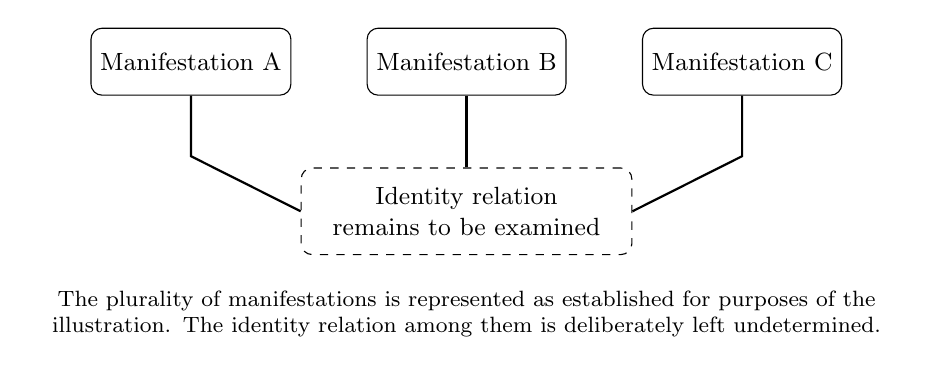
\begin{tikzpicture}[
    manifestation/.style={
        draw,
        rounded corners,
        minimum width=2.1cm,
        minimum height=0.85cm,
        align=center,
        font=\small
    },
    question/.style={
        draw,
        rounded corners,
        dashed,
        minimum width=4.2cm,
        minimum height=1.1cm,
        align=center,
        font=\small
    },
    relation/.style={
        thick,
        -
    }
]

\node[manifestation] (m1) at (-3.5,1.5) {Manifestation A};
\node[manifestation] (m2) at (0,1.5) {Manifestation B};
\node[manifestation] (m3) at (3.5,1.5) {Manifestation C};

\node[question] (identity) at (0,-0.4) {
    Identity relation\\
    remains to be examined
};

\draw[relation] (m1.south) -- (-3.5,0.3) -- (identity.west);
\draw[relation] (m2.south) -- (identity.north);
\draw[relation] (m3.south) -- (3.5,0.3) -- (identity.east);

\node[
    align=center,
    text width=0.9\textwidth,
    font=\footnotesize
] at (0,-1.7) {
    The plurality of manifestations is represented as established
    for purposes of the illustration. The identity relation among
    them is deliberately left undetermined.
};

\end{tikzpicture}

\caption{Plurality of Manifestations and the Unresolved Identity Relation}
\label{fig:manifestation-plurality-and-identity-scope}
\end{figure}

% =============================================================================
% END OF ILLUSTRATION IL01
% =============================================================================

The illustration distinguishes the plurality of
manifestations from the identity question associated
with them. It deliberately leaves the identity
relation unresolved: the diagrammatic grouping of
manifestations is not intended to assert that
they necessarily belong to one identity or to
multiple identities. Its purpose is to make visible
the gap between a manifestational description
and an identity conclusion.

The relation between manifestation and identity
therefore remains an independent ontological problem.
Any conclusion concerning identity must be supported
by grounds that address the identity relation itself,
rather than by the number, similarity, difference,
or grouping of manifestations alone.

% -----------------------------------------------------------------------------
\subsection{The Limit of Numerical Enumeration}

Numerical enumeration cannot provide an exhaustive
account of unity or plurality. Counting requires
a domain of enumeration, a criterion of distinction,
and a specification of what is being counted.
Different criteria may produce different numerical
descriptions of the same broader configuration.
A composition may be counted as one composed
subject while its components are counted as several
elements. A broader configuration may be counted
as one aggregate while several existents remain
distinguishable within it.

Such descriptions are not necessarily contradictory
because they may concern different subjects or
respects. Their compatibility, however, does not
mean that numerical classification is arbitrary.
A count may be precise within its intended domain.
Its limitation concerns the range of conclusions
that may legitimately be drawn from it.

Numerical variation does not by itself determine
the ontological number of identities. The criterion
of enumeration may identify components, material
units, relations, manifestations, or aggregates,
but the identity status of the counted items
requires a separate analysis. A count of several
components is not yet a count of several identities;
a count of one aggregate is not yet a count of
one identity.

The distinction is particularly important when
a numerical description is transferred from one
level of analysis to another. The fact that a
configuration is one under a criterion of
aggregation does not establish that it is one
under a criterion relevant to identity. Likewise,
the fact that several units are distinguished
under a material or relational criterion does
not establish that several identities are involved.

Numerical classification may therefore contribute
to ontological analysis, but it cannot replace it.
The ontological significance of a numerical result
must be established through an account of the
relation between the counted subject, the criterion
of enumeration, and the determination under
investigation.

% -----------------------------------------------------------------------------
\subsection{The Limit of Treating Unity and Plurality as Opposites}

Unity and plurality are often presented as
mutually exclusive alternatives. This opposition
becomes misleading when the relevant subject,
domain, and ontological respect are not specified.
A configuration may be unified in one respect
and plural in another. The unity of an aggregate
may coexist with the plurality of its components;
the unity of a source may coexist with the
plurality of its manifestations; and a broader
configuration involving multiple identities
may exhibit unity under a different determination.

These possibilities do not establish that every
form of unity and plurality can coexist without
qualification. If unity and plurality are attributed
to the same subject, in the same respect, under
the same conditions, their compatibility cannot
simply be assumed. The apparent opposition must
be examined to determine whether the claims
actually concern the same determination or whether
one of them changes its subject, scope, or criterion.

The distinction between respects is therefore
not a device for dissolving every contradiction.
It is a requirement for identifying the content
of each claim. If the subjects or respects differ,
the claims may be compatible. If they are identical,
a further account is required to determine whether
the predicates are genuinely incompatible or
whether the terms have been used in different senses.

Unity and plurality must consequently not be
treated as unrestricted logical opposites. Their
relation depends on what is unified, what is plural,
and the respect in which each determination is
asserted. A conclusion about compatibility or
incompatibility must follow from that analysis,
not from the words alone.

% -----------------------------------------------------------------------------
\subsection{The Limits of Reduction to One Ontological Respect}

Unity and plurality cannot be adequately examined
when all ontological determinations are reduced
to a single respect. Material constitution,
composition, structural organization, relational
determination, manifestation, and identity are
not interchangeable categories. They may be
related within an existent, but the relation
does not make their respective questions identical.

A plurality established in one of these respects
cannot automatically be transferred to another.
Material plurality does not necessarily establish
plurality of identity. Relational plurality does
not necessarily establish multiple existents.
Plurality of determinations does not necessarily
establish plurality of identities. Conversely,
unity in material constitution does not
automatically establish unity of identity, and
structural organization does not independently
prove that the organized subject has one identity.

Every inference across ontological respects
requires an account of the relation that makes
the inference legitimate. It is not enough to
point out that two determinations belong to
the same existent or configuration. Their
co-occurrence does not establish that one
determines the other. A relation of constitution,
dependence, realization, or manifestation may
be relevant, but its ontological significance
must be established rather than assumed.

The following diagram distinguishes several
respects in which unity or plurality may be
examined. It does not arrange them into a
hierarchy, nor does it assert that one respect
grounds or determines another.

% =============================================================================
% Project : THE_PHILOSOPHY_OF_VIABILITY
% Book    : Book I — Ontology of Viability
% Book ID : VS.B01
%
% File    : 4_ASSETS/diagrams/VS.B01.P01.C03.S08.SS12.P003.DG01.limits_of_inference_across_ontological_respects.tex
%
% Asset:
%   Diagram DG01 — Limits of Inference Across Ontological Respects
%
% Purpose :
%   To distinguish several ontological respects in which unity
%   and plurality may be examined, and to show that conclusions
%   established in one respect do not automatically transfer
%   to another.
%
% =============================================================================

\begin{figure}[htbp]
\centering

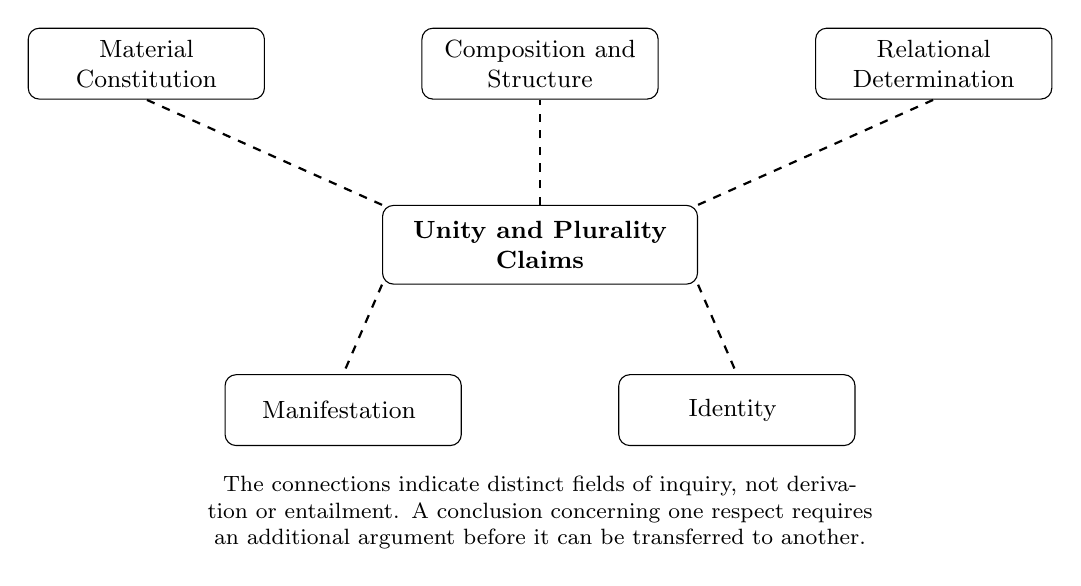
\begin{tikzpicture}[
    respect/.style={
        draw,
        rounded corners,
        align=center,
        minimum width=3.0cm,
        minimum height=0.9cm,
        font=\small
    },
    central/.style={
        draw,
        rounded corners,
        align=center,
        minimum width=4.0cm,
        minimum height=1.0cm,
        font=\small\bfseries
    },
    nonentailment/.style={
        dashed,
        thick,
        -
    }
]

\node[central] (inquiry) at (0,0) {
    Unity and Plurality\\
    Claims
};

\node[respect] (material) at (-5,2.3) {
    Material\\
    Constitution
};

\node[respect] (composition) at (0,2.3) {
    Composition and\\
    Structure
};

\node[respect] (relation) at (5,2.3) {
    Relational\\
    Determination
};

\node[respect] (manifestation) at (-2.5,-2.1) {
    Manifestation
};

\node[respect] (identity) at (2.5,-2.1) {
    Identity
};

\draw[nonentailment] (inquiry.north west) -- (material.south);
\draw[nonentailment] (inquiry.north) -- (composition.south);
\draw[nonentailment] (inquiry.north east) -- (relation.south);
\draw[nonentailment] (inquiry.south west) -- (manifestation.north);
\draw[nonentailment] (inquiry.south east) -- (identity.north);

\node[
    align=center,
    text width=0.92\textwidth,
    font=\footnotesize
] at (0,-3.4) {
    The connections indicate distinct fields of inquiry,
    not derivation or entailment. A conclusion concerning
    one respect requires an additional argument before
    it can be transferred to another.
};

\end{tikzpicture}

\caption{Limits of Inference Across Ontological Respects}
\label{fig:limits-of-inference-across-ontological-respects}
\end{figure}

% =============================================================================
% END OF DIAGRAM DG01
% =============================================================================

The diagram is an analytical map of possible
questions, not a complete inventory of the
ontology and not a causal or derivational model.
Its purpose is to prevent a determination
established in one respect from being transferred
to another without an explicit argument.

The reduction of all these questions to one
respect would conceal rather than resolve the
ontological problems under examination. A
satisfactory account must preserve the distinctions
while examining the relations among them.

% -----------------------------------------------------------------------------
\subsection{Unresolved Questions Concerning Identity and Number}

The restrictions established above leave several
ontological questions open. These questions are
not open merely because the relevant terms have
not yet been defined. They concern relations and
conditions that cannot be settled through unity,
plurality, or numerical classification alone.

Among the unresolved questions are:

\begin{itemize}
    \item Under what ontological conditions can
    an existent be established as involving
    exactly one identity?

    \item Under what conditions, if any, can
    multiple identities be involved in one
    existent or broader configuration?

    \item What grounds distinguish a plurality
    of manifestations from a plurality of identities?

    \item How are the identity boundaries of
    components related to the boundaries of
    a composition or aggregate?

    \item Can unity be established across
    different ontological respects without
    presupposing a single identity?

    \item What ontological relations connect
    a source with multiple manifestations
    without reducing source to manifestation
    or identity to source?

    \item What conditions make a distinction
    among elements relevant to identity rather
    than merely to material, structural,
    relational, or manifestational description?

    \item How should the possibility of identity
    plurality be assessed without presupposing
    that every existent has exactly one identity
    or that every differentiated configuration
    contains several identities?
\end{itemize}

These questions require further ontological
examination of identity, determination,
composition, relation, and manifestation.
They cannot be settled merely by defining
unity as oneness or plurality as multiplicity.
Nor should their openness be mistaken for
evidence that every proposed possibility
is equally established.

The present inquiry establishes restrictions
on what may be inferred. It does not claim
that the unresolved alternatives have already
been demonstrated. Their status must remain
provisional or open until the relevant
ontological grounds have been examined.

% -----------------------------------------------------------------------------
\subsection{Methodological Restrictions}

The analysis of unity and plurality must observe
a set of methodological restrictions. These
restrictions govern the formulation and evaluation
of ontological claims; they are not a substitute
for the substantive arguments required in each
particular case.

First, every claim of unity or plurality must
identify its subject. A statement that something
is one or multiple is incomplete if it does not
make clear what is being counted, unified,
distinguished, or related.

Second, the ontological respect and domain of
the claim must be specified. A conclusion
established concerning material constitution
cannot be transferred automatically to identity,
and a conclusion concerning manifestation
cannot be transferred automatically to source.

Third, numerical descriptions must not be treated
as complete ontological determinations. Counting
may be accurate within a domain while leaving
the identity status of the counted subject
unresolved.

Fourth, plurality of components, relations,
determinations, processes, or manifestations
must not be converted automatically into
plurality of identities. The ontological status
of the distinguished elements requires
independent examination.

Fifth, unity of source, aggregate, composition,
or structure must not be converted automatically
into unity of identity. Each form of unity
concerns a particular subject and respect.

Sixth, the distinction between unity and plurality
must not be used to impose a universal ontological
priority. Neither determination has been shown
to be an unrestricted ground from which all
other determinations can be derived.

Seventh, a distinction among respects must not
be introduced merely to protect a preferred
conclusion from criticism. The relevant respects
and their relations must be independently
specified, and apparent contradictions must
be examined rather than dismissed.

The methodological requirements and the
conclusions they restrict are summarized in
Table~\ref{tab:methodological-limits-of-unity-and-plurality}.

% =============================================================================
% Project : THE_PHILOSOPHY_OF_VIABILITY
% Book    : Book I — Ontology of Viability
% Book ID : VS.B01
%
% File    : 4_ASSETS/tables/VS.B01.P01.C03.S08.SS13.P003.TL01.methodological_limits_of_unity_and_plurality.tex
%
% Asset:
%   Table TL01 — Methodological Limits of Unity and Plurality
%
% Purpose :
%   To summarize the principal restrictions governing claims
%   about unity, plurality, and their implications for identity.
%
% =============================================================================

\begin{table}[htbp]
\centering
\caption{Methodological Limits of Unity and Plurality}
\label{tab:methodological-limits-of-unity-and-plurality}
\footnotesize
\renewcommand{\arraystretch}{1.2}

\begin{tabularx}{\textwidth}{
    @{}
    p{0.24\textwidth}
    X
    p{0.32\textwidth}
    @{}
}
\toprule
\textbf{Analytical Requirement} &
\textbf{Restriction} &
\textbf{Inference Not Licensed by Itself}
\\
\midrule

Specify the subject &
Identify what is unified, plural, counted, or distinguished. &
Unity of one subject establishes unity of another subject.
\\

Specify the respect &
Identify the ontological determination under examination. &
Material, relational, or manifestational plurality establishes identity plurality.
\\

Specify the domain &
Identify the range within which the claim is valid. &
A local numerical result applies to every ontological domain.
\\

Specify the criterion &
Identify what counts as one or multiple. &
Numerical classification determines ontological identity-number.
\\

Preserve conceptual distinctions &
Keep source, aggregate, composition, structure, manifestation, and identity distinct. &
Unity or plurality in one category settles another category.
\\

Establish cross-respect relations &
Provide grounds for transferring a conclusion between respects. &
Co-occurrence of determinations establishes entailment.
\\

Preserve unresolved questions &
Do not convert insufficient evidence into a universal conclusion. &
Failure to prove plurality establishes singular identity, or vice versa.
\\

\bottomrule
\end{tabularx}
\end{table}

% =============================================================================
% END OF TABLE TL01
% =============================================================================

These requirements define conditions for
responsible ontological inference. They do
not constitute a universal definition of
unity, plurality, or identity. Nor do they
settle the final structure of every existent.
Their function is to ensure that an argument
does not claim more than its premises and
ontological grounds establish.

% -----------------------------------------------------------------------------
\subsection{Conclusion: The Scope and Limits of Unity and Plurality}

Unity and plurality are indispensable for
examining the ontological organization of
existents. Their significance, however,
does not make either an unrestricted
explanation of identity, source, composition,
aggregate, structure, or manifestation.

Unity does not establish numerical singularity
or exactly one identity. Plurality does not
establish multiple identities. The unity
of a source or aggregate does not automatically
determine the identity of what is related
to it, and the plurality of components or
manifestations does not automatically
determine the plurality of identities involved.

The analysis has also established that
conclusions must remain within the scope
of the subject and respect for which they
were justified. A determination established
in one ontological respect may be relevant
to another, but relevance does not establish
entailment. The relation must be demonstrated
through an argument appropriate to the
ontological questions involved.

The unresolved questions concerning
identity-number and the relations among
identities must therefore remain open
where the available grounds do not settle
them. This openness is not an endorsement
of every possible answer. It is a refusal
to treat an unsupported inference as an
established ontological result.

The chapter's final section will synthesize
the distinctions developed throughout
the inquiry. It will identify the results
that can be retained, the claims whose
scope has been restricted, and the questions
that remain unresolved, without converting
those results into a premature universal
theory of unity, plurality, or identity.

% =============================================================================
% END OF SECTION 08 OF CHAPTER 03
% =============================================================================

% ------------------------------------------------------------
% SECTION 09
% ------------------------------------------------------------

% =============================================================================
% Section 09 — Synthesis of Unity and Plurality
% Book I — Ontology of Viability
% Chapter 03 — Unity and Plurality
%
% Purpose:
%   To synthesize the ontological distinctions established
%   throughout the chapter and clarify the results that can
%   be retained without imposing a premature resolution
%   of the relation between unity, plurality, and identity.
%
% Conceptual Policy:
%   1. Unity and plurality remain distinct ontological determinations.
%   2. Neither unity nor plurality receives universal priority.
%   3. Unity is not equivalent to singularity.
%   4. Plurality is not equivalent to multiplicity alone.
%   5. Source, aggregate, composition, and identity remain distinct.
%   6. Multiplicity of manifestations does not establish
%      plurality of identities.
%   7. Unity of an aggregate does not establish unity of identity.
%   8. The number of identities remains an independent
%      ontological question.
%
% =============================================================================

\section{Synthesis of Unity and Plurality}
\label{sec:synthesis-of-unity-and-plurality}

% -----------------------------------------------------------------------------
\subsection{The Result of the Inquiry}

The preceding sections have examined unity
and plurality as fundamental but non-equivalent
determinations within the ontology of existents.

The inquiry has not sought to establish
one as the universal foundation of the other.

Rather, it has examined the conditions
under which unity and plurality can be
attributed, the subjects to which such
attributions apply, and the limits of
the inferences that can be drawn from them.

The principal result is that unity and
plurality cannot be adequately understood
through numerical description alone.

Nor can either be reduced to composition,
source, manifestation, or identity.

Their ontological significance depends
on the subject and respect under examination.

The chapter therefore establishes a framework
of distinctions through which claims about
unity and plurality can be evaluated without
prematurely determining the number or
organization of identities.

% -----------------------------------------------------------------------------
\subsection{Unity and Plurality as Distinct Determinations}

Unity and plurality must first be retained
as distinct determinations.

Unity concerns the ontological respect
in which a subject is considered unified.

Plurality concerns the presence of
distinguishable multiple subjects or
elements within a specified domain
and respect.

Their distinction does not imply that
they are universally incompatible.

A subject may exhibit unity in one respect
while involving plurality in another.

Likewise, a plurality of entities may
participate in a configuration that
exhibits unity under a different
ontological determination.

The relation between unity and plurality
must therefore be established through
the identification of their respective
subjects and domains.

Neither concept can be applied without
qualification to every aspect of an existent.

% -----------------------------------------------------------------------------
\subsection{Unity and Singularity}

One of the principal distinctions
established in this chapter concerns
the non-equivalence of unity and
numerical singularity.

Unity is not simply the condition
of being numerically one.

Singularity concerns numerical
determination within a specified
domain of enumeration.

Unity concerns an ontological respect
in which something is unified.

Consequently:

\[
\text{Unity}
\neq
\text{Numerical Singularity}
\]

Numerical oneness does not independently
establish unity of identity.

Likewise, unity does not automatically
establish that exactly one identity
is involved.

This distinction prevents the numerical
classification of an existent from
being treated as a complete account
of its ontological identity.

% -----------------------------------------------------------------------------
\subsection{Unity of Identity and Unity of Source}

The inquiry has also distinguished
unity of identity from unity of source.

A source may be considered one in
a particular respect without this
determining the identity of everything
related to it.

A common source does not automatically
establish one identity among its
manifestations or related entities.

Conversely, plurality among manifestations
does not automatically establish plurality
of sources.

Source relations and identity relations
must therefore remain analytically distinct.

The ontological significance of a source
cannot be exhausted by its relation
to the number of manifestations or
entities associated with it.

% -----------------------------------------------------------------------------
\subsection{Unity of Aggregate and Unity of Identity}

Unity of aggregate must likewise be
distinguished from unity of identity.

An aggregate may constitute a unified
configuration through relations among
its components.

However, the unity of that configuration
does not independently determine whether
one or multiple identities are involved.

The components may retain ontological
distinctions that cannot be eliminated
merely by describing them as parts
of one aggregate.

Similarly, the existence of multiple
components does not automatically
negate every form of unity within
the aggregate.

The following distinction remains
fundamental:

\[
\text{Unity of Aggregate}
\neq
\text{Unity of Identity}
\]

The relation between aggregate and
identity requires an independent
ontological account.

% -----------------------------------------------------------------------------
\subsection{Plurality of Components, Relations, and Manifestations}

The chapter has distinguished plurality
of elements from plurality of identities.

An existent may involve multiple:

\begin{itemize}
    \item Components.
    \item Determinations.
    \item Relations.
    \item Manifestations.
    \item Processes.
    \item Configurations.
\end{itemize}

The presence of these forms of multiplicity
does not automatically establish that
multiple identities are involved.

Multiplicity is therefore not equivalent
to plurality of identities.

The distinction is especially important
because different ontological respects
may contain different forms of plurality
without requiring that they be transferred
to the domain of identity.

The number and organization of identities
must be examined independently of the
mere number of components, relations,
or manifestations.

% -----------------------------------------------------------------------------
\subsection{Plurality of Identities and Composition}

The possibility of multiple identities
must remain distinct from the plurality
of components within a composition.

A composition may contain multiple
components without each component
constituting a distinct identity.

Conversely, the possibility of multiple
identities within a broader configuration
cannot be excluded merely because
that configuration is described
as one composition.

Composition may be relevant to the
determination of identity, but it cannot
serve as its universal or exclusive
foundation.

The relation between identity and
composition must therefore be examined
without assuming that their boundaries
necessarily coincide.

% -----------------------------------------------------------------------------
\subsection{The Independence of Ontological Questions}

The distinctions developed in this
chapter establish that several questions
must not be collapsed into one another.

In particular, the following questions
are analytically distinct:

\begin{enumerate}
    \item Whether a subject is unified
    in a specified ontological respect.

    \item Whether something is numerically
    singular within a particular domain.

    \item Whether a plurality of components
    constitutes one aggregate.

    \item Whether multiple entities share
    a common source.

    \item Whether an existent possesses
    one identity or involves multiple
    identities.

    \item Whether multiple manifestations
    belong to one identity or to distinct
    identities.

    \item Whether a composition and the
    identities involved in it have
    corresponding ontological boundaries.
\end{enumerate}

These questions may be related,
but their relations must be established
rather than assumed.

An answer to one does not automatically
provide an answer to the others.

This analytical independence is necessary
to prevent the reduction of identity
to numerical classification, source,
composition, or manifestation.

% -----------------------------------------------------------------------------
\subsection{A Framework for Examining Unity and Plurality}

The results of the chapter can be
organized through a set of methodological
requirements.

Every claim concerning unity or plurality
must identify:

\begin{itemize}
    \item The subject to which the claim applies.
    \item The ontological respect being examined.
    \item The domain within which the claim is made.
    \item The distinctions required to identify
    the relevant units or elements.
    \item The limits of the inference being drawn.
\end{itemize}

These requirements do not constitute
a universal definition of unity or
plurality.

They establish the minimum conditions
for making such claims without confusing
different ontological determinations.

The framework also prevents a determination
established in one respect from being
transferred to another without justification.

For example, material unity cannot
automatically be converted into unity
of identity, just as relational plurality
cannot automatically be converted into
plurality of identities.

% -----------------------------------------------------------------------------
\subsection{Established Results and Unresolved Questions}

The inquiry supports several conclusions
that can be retained as results of
the present chapter.

First, unity and plurality are not
equivalent to numerical singularity
and numerical multiplicity.

Second, unity and plurality are not
universally mutually exclusive.

Third, unity of source, aggregate,
or composition does not independently
establish unity of identity.

Fourth, plurality of components,
relations, or manifestations does
not independently establish plurality
of identities.

Fifth, identity cannot be reduced
to numerical classification or
compositional organization.

These conclusions establish restrictions
on ontological inference.

They do not, however, settle every
question concerning the number of
identities within an existent.

Several issues remain open:

\begin{itemize}
    \item The ontological conditions
    under which singular identity
    is established.

    \item The conditions under which
    multiple identities may be involved
    in one broader configuration.

    \item The relation between identity
    boundaries and compositional boundaries.

    \item The ontological relation between
    a source and its multiple manifestations.

    \item The conditions under which
    unity may extend across different
    ontological respects.

    \item The possibility and limits
    of identity plurality within an
    existent or a broader configuration.
\end{itemize}

These questions require further analysis
and must not be resolved through
assumptions introduced by the concepts
of unity or plurality themselves.

% -----------------------------------------------------------------------------
\subsection{The Ontological Significance of the Distinctions}

The distinctions established in this
chapter are not merely terminological.

They prevent different ontological
questions from being treated as though
they were interchangeable.

Without these distinctions, numerical
oneness may be mistaken for identity
unity, aggregate unity for singular
identity, or manifestational plurality
for identity plurality.

Such reductions would obscure the
ontological structure of the problems
under examination.

The distinction between unity and
plurality therefore provides a necessary
condition for the further analysis
of identity and manifestation.

It preserves the possibility that
different ontological respects may
exhibit different forms of unity and
plurality without requiring their
reduction to one determination.

This result is methodological and
ontological in significance.

It clarifies what can be established
and what remains to be demonstrated.

% -----------------------------------------------------------------------------
\subsection{Transition to the Further Ontology of Identity}

The present chapter has established
that unity and plurality cannot
independently determine the number
or structure of identities.

The inquiry into identity must therefore
proceed without treating unity as
proof of singular identity or plurality
as proof of multiple identities.

The next stages of the ontology must
examine the conditions through which
identity is constituted, distinguished,
and related to the other determinations
of an existent.

Such an examination must preserve
the distinctions established here
while investigating the ontological
relations that remain unresolved.

The results of this chapter consequently
provide a conceptual restriction
and a methodological foundation
for the further development of
the ontology of viability.

% =============================================================================
% End of Section 09
% =============================================================================

% ------------------------------------------------------------
% CHAPTER CONCLUSION
% ------------------------------------------------------------

\section*{Chapter Conclusion}
\addcontentsline{toc}{section}{Chapter Conclusion}

This chapter has examined unity and plurality as
distinct but interrelated ontological problems within
the ontology of viability.

The analysis has established that assertions of unity
and plurality require specification of their subject
and respect. Without such specification, it is not
possible to determine whether a claim concerns identity,
source, aggregate, composition, determination, relation,
or manifestation.

The chapter has also maintained the distinction between
unity of identity, unity of source, and unity of aggregate.
These forms of unity cannot be assumed to possess the
same ontological meaning or to entail one another
without further argument.

Likewise, plurality of components, relations, determinations,
or manifestations cannot be treated as sufficient evidence
for plurality of identities. The relation between
multiplicity within an existent and the possible
multiplicity of identities remains a question requiring
independent examination.

The distinction between unity and singularity further
prevents the assumption that every assertion of unity
necessarily establishes numerical singularity. Unity
and singularity must therefore remain analytically
distinguishable.

The chapter has not established a universal rule according
to which every existent must possess exactly one identity,
nor has it established that an existent may necessarily
possess multiple identities. These possibilities have
been retained as subjects of ontological inquiry rather
than treated as predetermined conclusions.

Consequently, the analysis provides a framework for
examining the relations between identity, unity, plurality,
source, aggregate, and composition without reducing
any of these concepts to another.

The question of how unity and plurality are ultimately
grounded within the broader architecture of the ontology
of viability remains open for further development.
The distinctions established here provide the basis
for subsequent investigations into the ontological
determinations and manifestations of an existent.

% ============================================================
% END OF CHAPTER 03
% ============================================================
